% Options for packages loaded elsewhere
\PassOptionsToPackage{unicode}{hyperref}
\PassOptionsToPackage{hyphens}{url}
\PassOptionsToPackage{dvipsnames,svgnames,x11names}{xcolor}
%
\documentclass[
  11pt,
]{book}
\title{Dispense modulo univariata}
\author{Giorgio Marrubini e Camillo Melzi}
\date{}

\usepackage{amsmath,amssymb}
\usepackage{lmodern}
\usepackage{iftex}
\ifPDFTeX
  \usepackage[T1]{fontenc}
  \usepackage[utf8]{inputenc}
  \usepackage{textcomp} % provide euro and other symbols
\else % if luatex or xetex
  \usepackage{unicode-math}
  \defaultfontfeatures{Scale=MatchLowercase}
  \defaultfontfeatures[\rmfamily]{Ligatures=TeX,Scale=1}
\fi
% Use upquote if available, for straight quotes in verbatim environments
\IfFileExists{upquote.sty}{\usepackage{upquote}}{}
\IfFileExists{microtype.sty}{% use microtype if available
  \usepackage[]{microtype}
  \UseMicrotypeSet[protrusion]{basicmath} % disable protrusion for tt fonts
}{}
\makeatletter
\@ifundefined{KOMAClassName}{% if non-KOMA class
  \IfFileExists{parskip.sty}{%
    \usepackage{parskip}
  }{% else
    \setlength{\parindent}{0pt}
    \setlength{\parskip}{6pt plus 2pt minus 1pt}}
}{% if KOMA class
  \KOMAoptions{parskip=half}}
\makeatother
\usepackage{xcolor}
\IfFileExists{xurl.sty}{\usepackage{xurl}}{} % add URL line breaks if available
\IfFileExists{bookmark.sty}{\usepackage{bookmark}}{\usepackage{hyperref}}
\hypersetup{
  pdftitle={Dispense modulo univariata},
  pdfauthor={Giorgio Marrubini e Camillo Melzi},
  colorlinks=true,
  linkcolor={Maroon},
  filecolor={Maroon},
  citecolor={Blue},
  urlcolor={Blue},
  pdfcreator={LaTeX via pandoc}}
\urlstyle{same} % disable monospaced font for URLs
\usepackage[left=2cm, right=2.5cm, top=2.5cm, bottom=2.5cm]{geometry}
\usepackage{longtable,booktabs,array}
\usepackage{calc} % for calculating minipage widths
% Correct order of tables after \paragraph or \subparagraph
\usepackage{etoolbox}
\makeatletter
\patchcmd\longtable{\par}{\if@noskipsec\mbox{}\fi\par}{}{}
\makeatother
% Allow footnotes in longtable head/foot
\IfFileExists{footnotehyper.sty}{\usepackage{footnotehyper}}{\usepackage{footnote}}
\makesavenoteenv{longtable}
\usepackage{graphicx}
\makeatletter
\def\maxwidth{\ifdim\Gin@nat@width>\linewidth\linewidth\else\Gin@nat@width\fi}
\def\maxheight{\ifdim\Gin@nat@height>\textheight\textheight\else\Gin@nat@height\fi}
\makeatother
% Scale images if necessary, so that they will not overflow the page
% margins by default, and it is still possible to overwrite the defaults
% using explicit options in \includegraphics[width, height, ...]{}
\setkeys{Gin}{width=\maxwidth,height=\maxheight,keepaspectratio}
% Set default figure placement to htbp
\makeatletter
\def\fps@figure{htbp}
\makeatother
\setlength{\emergencystretch}{3em} % prevent overfull lines
\providecommand{\tightlist}{%
  \setlength{\itemsep}{0pt}\setlength{\parskip}{0pt}}
\setcounter{secnumdepth}{5}
\usepackage{booktabs}
\usepackage{amsmath}
\usepackage[italian]{babel}\addto\extrasitalian{
  \def\figureautorefname{Figura}
  \def\chapterautorefname{Capitolo}
  \def\sectionautorefname{Paragrafo}
  \def\subsectionautorefname{Paragrafo}
  \def\subsubsectionautorefname{Paragrafo}
  \def\equationautorefname{Equazione}
  \def\tableautorefname{Tabella}}
\usepackage{arydshln}
\ifLuaTeX
  \usepackage{selnolig}  % disable illegal ligatures
\fi
\usepackage[]{natbib}
\bibliographystyle{plainnat}

\begin{document}
\maketitle

{
\hypersetup{linkcolor=}
\setcounter{tocdepth}{1}
\tableofcontents
}
\hypertarget{section}{%
\chapter*{}\label{section}}
\addcontentsline{toc}{chapter}{}

\hypertarget{glossario}{%
\chapter*{Glossario minimo}\label{glossario}}
\addcontentsline{toc}{chapter}{Glossario minimo}

Le voci seguenti sono in ordine alfabetico e riportano alcune definizioni di termini e concetti di base che ricorrono nelle dispense.
Le definizioni sono tratte dai riferimenti citati in bibliografia.
\citep{legarzantine2014, everittb.s.skrondala.2010, wonnacottt.h.wonnacottr.j.2002}

\textbf{Aleatorio, campione a., evento a., intervallo a., variabile a.}\\
Il termine aleatorio è sinonimo di casuale.
Deriva da ``alea'' che in latino significa dado.
Quindi aleatorio è aggettivo di un campione, un evento o altro la cui natura è legata al caso (v. anche la voce \emph{caso, casuale}).

\textbf{Analisi di correlazione}\\
Verifica del fatto che due variabili siano correlate tra loro.
V. \emph{Correlazione}.

\textbf{Analisi di regressione}\\
Definizione del modello funzionale per cui una proprietà Y dipende da un fattore X e quindi che valga la relazione Y = f(X).
Nel caso di più fattori, X\textsubscript{1}, X\textsubscript{2}, \ldots, X\textsubscript{n}, si parla di regressione multipla e si verifica quindi la validità della relazione Y = f(X\textsubscript{1}, X\textsubscript{2}, \ldots, X\textsubscript{n}).

\textbf{Autocorrelazione} v. anche \emph{Correlazione}.
L'autocorrelazione è il grado di dipendenza tra i valori che assumono le variabili in ascissa.

\textbf{Campionario, media c., varianza c.}\\
Campionario è detto di proprietà relativa al campione.

\textbf{Caso, casuale}\\
Il caso è un termine con cui si indica un evento che si verifica indipendentemente (almeno in apparenza) da una causa oggettiva, oppure un evento di cui non si conoscono le cause.

\textbf{Confidenza, intervallo di c., livello di c.}\\
In statistica è sinonimo di ``fiducia''.
Indica la probabilità o grado di fiducia che la stima di un parametro sulla base di un campione (per es. la media) sia una buona approssimazione del parametro della popolazione.
Più in dettaglio, fissato un valore di probabilità 1-\(\alpha\) (con 0\textless{} \(\alpha\) \textless1), detto \emph{livello di di confidenza} (es. 1-\(\alpha\) = 95\%), \emph{l'intervallo di confidenza} è l'intervallo {[}\(\theta_1\), \(\theta_2\){]} all'interno del quale si trova il valore del parametro \(\theta\) da stimare, con probabilità 1-\(\alpha\).
Il numero \(\alpha\) è detto \emph{livello di significatività} (v. anche \emph{Significatività}) ed esprime la probabilità di compiere un errore cosiddetto di I tipo, affermando che il valore del parametro da stimare non appartiene all'intervallo di confidenza quando in realtà ciò è vero (rifiuto l'ipotesi nulla \(H_0\) quando questa è vera).

\textbf{Correlazione} \emph{c.~lineare, c.~seriale, c.~multipla}\\
Legame di interdipendenza tra due o più variabili statistiche quantitative.
Tra due variabili, esiste correlazione, se al variare dell'una anche l'altra varia in modo non casuale.\\
Se il legame tra due variabili è approssimabile con una funzione lineare, cioè rappresentabile mediante una retta, si parla di c
. lineare o di collinearità
.

\textbf{Covarianza}\\
Legame di interdipendenza tra due variabili aleatorie.

\textbf{Deterministico, modello d.}\\
Un modello deterministico è una equazione che a partire da certe condizioni iniziali note (es. una legge fisica) consente di conoscere con buona approssimazione il risultato del fenomeno in osservazione (es. legge di caduta dei gravi: lascio cadere un grave e osservo che esso raggiunge il suolo con una certa accelerazione).

\textbf{Disegno}\\
\emph{d.~sperimentale, d.~fattoriale, d.~di miscele, d.~fattoriale frazionario, d.~D-ottimale, d.~di screening}\\
Sinonomo di progetto, piano di studio, piano degli esperimenti
.

\textbf{Economia degli effetti, principio di} \emph{Sparsity of effects principle} Principio basato sulla osservazione empirica, fino ad oggi mai confutata, secondo cui la maggior parte dei sistemi (chimici e fisici) è regolata da pochi effetti principali e interazioni di ordine 2; la maggior parte degli effetti riconducibili a interazioni di ordine superiore a 2 è trascurabile.
\citep{lietal.2006}\citep{bergquistetal.2011}

\textbf{Effetto}\\
Variazione della risposta sperimentale che è prodotta da uno o più fattori, o dalle loro interazioni.

\textbf{Fattore}\\
Ognuna delle m variabili aleatorie, non correlate tra loro, che si ricavano da un insieme più numeroso di k (k\textgreater m) variabili che si suppongono interdipendenti.

\textbf{Intervallo di confidenza, v. confidenza}

\textbf{Ipotesi, i. statistica}\\
Enunciato formulato per indagarne le conseguenze a prescindere dalla sua verità fattuale.
Nello studio di un problema, l'ipotesi è la proprietà che si suppone vera e dalla quale mediante una verifica o una dimostrazione obiettiva, si deducono altre proprietà.
In statistica, nella procedura di verifica delle ipotesi (test di ipotesi), l'ipotesi nulla \(H_0\) (\emph{null hypothesis}), è l'ipotesi di partenza che costituisce la proposizione espressa sotto forma di equazione verificabile quantitativamente che si formula prima di predisporre un esperimento e analizzare i risultati di un test statistico.
Accanto alla ipotesi nulla è formulata la sua negazione denominata ipotesi alternativa e indicata con \(H_1\).

\textbf{Livello di confidenza, v. Confidenza}

\textbf{Minimi quadrati, metodo dei m.q.}\\
Metodo di stima usato nei modelli di regressione in cui una variabile dipendente y è espressa attraverso una funzione (lineare o non lineare) di una o più variabili indipendenti.
Il metodo dei minimi quadrati consiste nello scegliere come stime dei parametri che figurano nell'equazione i valori che rendono mimima la somma dei quadrati delle differenze tra i valori della variabile y stimata come dipendente (valori osservati sperimentalmente \(y_i\), in corrispondenza dei valori di \(x-i\)) e quelli stimati mediante la funzione.
Per fissare le idee, se (\(x_i\), \(y_i\)) sono \emph{n} coppie di osservazioni sulle variabili X e Y e la relazione ipotizzata tra X e Y è lineare, la funzione che lega le due variabili è Y = a + bX.
In corrispondenza di ogni valore \(x_i\) si ha un valore reale osservato \(y_i\) e un valore teorico, detto valore \emph{atteso} \(\hat{y_i} = a + bx_i\).
Tra ogni valore atteso e ogni valore osservato c'è uno \emph{scarto d} calcolato dalla formula: \(d_i=|y_i-\hat{y_i}| =|y_i-(a + bx_i)|\).
La somma dei quadrati di tutti gli scarti \(d_i\) è una misura della distanza tra il modello teorico scelto e i dati osservati.
Il metodo di stima dei minimi quadrati porta quindi a scegliere a e b in modo tale che sia minima la quantità \[\sum_{i=1}^{n} [y_i-(a+bx_i)]^2\]

La retta individuata dai parametri a e b così ottenuti prende il nome di \emph{retta dei minimi quadrati} o \emph{retta di regressione}.
Il principio dei minimi quadrati assicura di determinare la funzione che con maggiore probabilità si adatta ai dati rilevati.
Il metodo di calcolo dei coefficienti a e b consiste in un procedimento di approssimazioni successive che, partendo dal valore della media dei valori osservati, attraverso il calcolo degli scarti e successive correzioni della media, permette di stabilire il valore più probabile della stima di a e b e fornisce un indice della sua precisione (lo scarto più piccolo appunto).

\textbf{Parametro}\\
Sinonimo di dato numerico, numero.

\textbf{Percentile, v. quantile}

\textbf{Probabilità}\\
Valutazione numerica attribuita al possibile verificarsi di un evento aleatorio, cioè casuale.

\textbf{Quantile}\\
Indice di posizione che fornisce informazioni sulla struttura della distribuzione di una serie di dati.
In una successione di numeri posti in ordine non crescente o non decrescente i quantili dividono la successione in \emph{n} gruppi contenenti un uguale numero di osservazioni.
In particolare, si parla di \emph{quartile}, \emph{decile} o \emph{percentile} a seconda che si ottengano quattro, dieci o cento gruppi di dati.
Se i dati sono ordinati (ad es. dal più piccolo al più grande), i \emph{percentili} sono i 99 valori che dividono l'insieme dei dati in 100 intervalli (da 1 a 100) di uguale numerosità.
Il cinquantesimo percentile coincide con la mediana della distribuzione.
I percentili, come i decili e i quartili fanno parte del concetto generale di suddivisione di una distribuzione ordinata in q parti uguali delle \emph{quantili}. Quindi ad esempio se la serie di dati in esame è \(x_1\), \(x_2\), \ldots, \(x_9\), ordinata dal numero più piccolo al numero più grande, allora \(x_1\) è il primo decile, e il 10\% dei dati è compreso tra 0 e \(x_1\), mentre \(x_9\) è il 9° decile e il 90\% dei dati è minore di \(X_9\).

\textbf{Risposta}\\
\emph{r. sperimentale, r. di un sistema, r. di un apparecchio, r. di un dispositivo, r. di un esperimento}, il modo con cui il sistema (apparecchio, dispositivo, esperimento) esplica il processo in osservazione, al variare delle condizioni di operazione.

\textbf{Scarto, s. interquartile, s. quadratico medio}\\
In statistica si indica con \emph{scarto} il valore di una differenza, per esempio tra un valore osservato e il valore calcolato da una funzione di regressione, oppure tra un valore assunto da una variabile e un valore fisso (es. media o mediana).
Il termine \emph{scarto} può essere usato anche per indicare una misura dell'insieme di più differenze: in questo caso il termine \emph{scarto} è seguito da da aggettivi che specificano come sia stata realizzata la sintesi delle differenze e assume il significato di un indice di variabilità come ad esempio lo \emph{scarto} o \emph{differenza interquartile}, che è la differenza tra il terzo e il primo quartile di una distribuzione (\(Q_3\)-\(Q_1\)).
Lo \emph{scarto quadratico medio} è la varianza.

\textbf{Significatività}\\
\emph{livello di s.}\\
Probabilità di commettere un errore di prima specie in un test di verifica di ipotesi, vale a dire che la s
. è la probabilità di rifiutare l'ipotesi nulla quando questa è vera
. E' un numero indicato con la lettera dell'alfabeto greco \(\alpha\), generalmente fissato pari a 0.05 (e si dice allora che il test è significativo al livello del 5\%), oppure a 0.01 (test significativo al livello dell'1\%)
. Nella stima di un parametro sulla base di un campione, il livello di significatività \(\alpha\) è strettamente legato al livello di probabilità dell'intervallo di confidenza prefissato in quanto ne è il complemento a 1 (equivalente a dire al 100\%)
.

\textbf{Statistica}\\
1) In generale, disciplina della matematica che si occupa della analisi quantitativa delle osservazioni di un qualsiasi fenomeno soggetto a variazione.
In particolare, la statistica è la scienza che si occupa della raccolta, della analisi, della interpretazione, della presentazione e della organizzazione di dati numerici.

\begin{enumerate}
\def\labelenumi{\arabic{enumi})}
\setcounter{enumi}{1}
\tightlist
\item
  Risultati numerici di una analisi di dati (es. la deviazione standard relativa percentuale di una serie di misure, RSD\%)
\item
  Valore numerico di un parametro statistico (es. il valore di t calcolato per una serie di dati).
\end{enumerate}

\textbf{Stima, s. puntuale, s. per intervallo}\\
La stima è la assegnazione sulla base dei dati campionari di uno o più valori numerici ad un parametro ignoto che caratterizza una popolazione (es. statura media della popolazione maschile italiana nel 1999).
In statistica inferenziale, si distingue tra i valori della popolazione (detti parametri) e i corrispondenti valori numerici che si ricavano dal campione (che rappresentano le stime dei parametri di cui sopra).
Quindi sulla base di un campione aleatorio si vuole trovare un valore, o un insieme di valori, che sia la migliore approssimazione possibile del valore incognito del parametro della popolazione.
Quando è assegnato un unico valore si parla di \emph{stima puntuale}; se invece è assegnato un insieme di valori, si parla di \emph{stima per intervallo}.

\textbf{Test di ipotesi, v. Ipotesi}

\textbf{Trattamento}\\
Dato un fattore X, stabiliti i due livelli -1 e +1 entro cui esso può variare, si definiscono trattamenti i due esperimenti in cui X assume i valori assegnati, X = -1 o X = +1.
Per più fattori, X\textsubscript{1}, X\textsubscript{2}, \ldots, X\textsubscript{n}, ogni trattamento corrisponde a una combinazione dei livelli (±1) degli n fattori.

\textbf{Variabile}, \emph{v. dipendente, v. indipendente}\\
Ente che può identificarsi con ciascuno degli elementi di un insieme assegnato.
Una variabile può assumere tutti i valori all'interno di tale insieme.
In una equazione in una incognita, la variabile è l'incognita stessa.
La notazione funzionale indica il valore di una variabile dipendente al variare di una o più variabili indipendenti, come ad esempio in y = f(x), in cui x è la variabile indipendente e y la variabile dipendente da x secondo la relazione funzionale ``f''.
Se due variabili sono \emph{statisticamente} indipendenti si dice anche che esse sono \emph{incorrelate} (v. \emph{Correlazione}).

\textbf{Verifica delle ipotesi, v. Ipotesi}

\hypertarget{statistica-descrittiva}{%
\chapter{Statistica descrittiva}\label{statistica-descrittiva}}

Si illustrano nel seguito alcuni strumenti della statistica descrittiva di uso molto comune per visualizzare e riassumere dati.

Dal menu ``Dati'' alla voce ``Esempi Master'' si può scegliere il file ``Resa estrattiva'' e vedere cosa contiene. Si tratta di una serie di dati, ottenuti dall'analisi di estratti vegetali. Il dataset consiste in 10 misure della resa estrattiva di un metodo di isolamento di polifenoli da infusi acquosi di Dittamo cretese (Origanum dictamus, meglio noto come Cretan tea), una pianta aromatica e medicinale tradizionalmente considerata un rimedio generale per molti disturbi (dalla stanchezza ai disturbi digestivi, alla capacità di agire come disinfettante e cicatrizzante).

\begin{figure}

{\centering 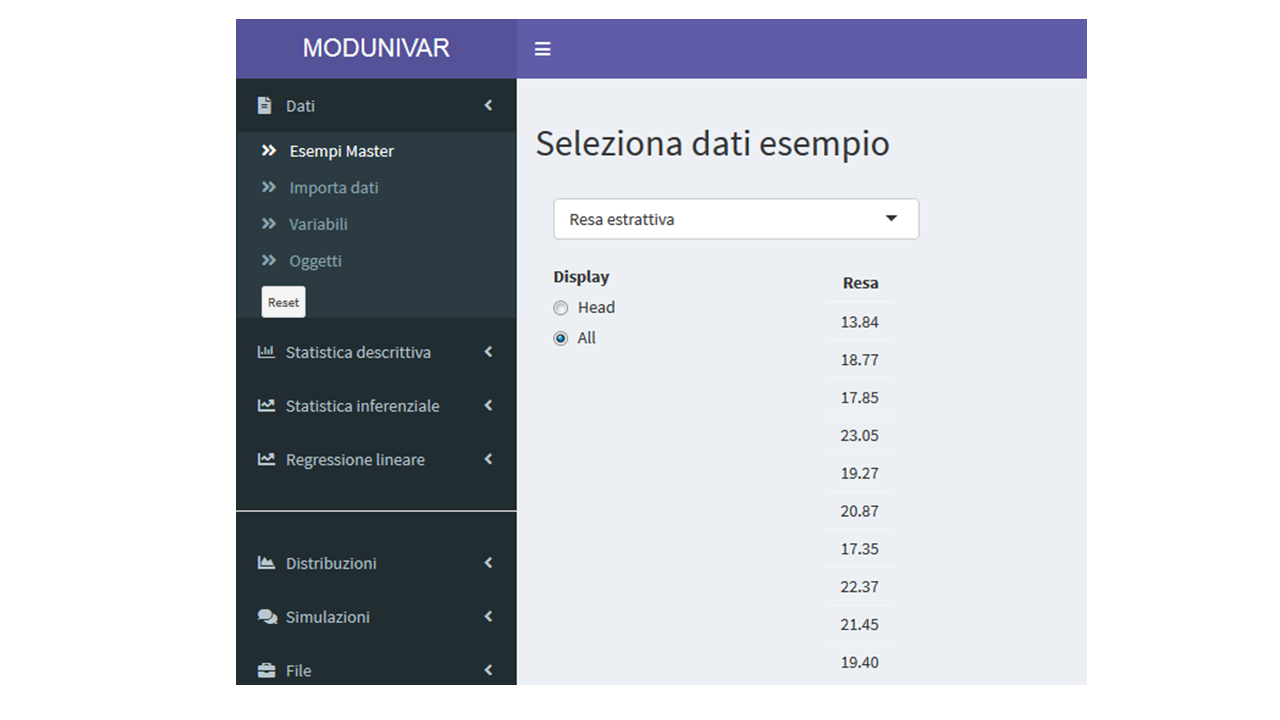
\includegraphics[width=1\linewidth]{Immagini/Descrittiva/1_Resa_estrattiva} 

}

\caption{Il dataset Resa estrattiva tra gli esempi didattici a disposizione per le lezioni del Master ECAIF}\label{fig:sd1}
\end{figure}

La prima funzione descrittiva che di solito si usa è quella di mettere i dati in una tabella: nel menu ``statistica descrittiva'' la voce ``Vedi dati'' consente di stampare in una tabella le misure.

\begin{figure}

{\centering 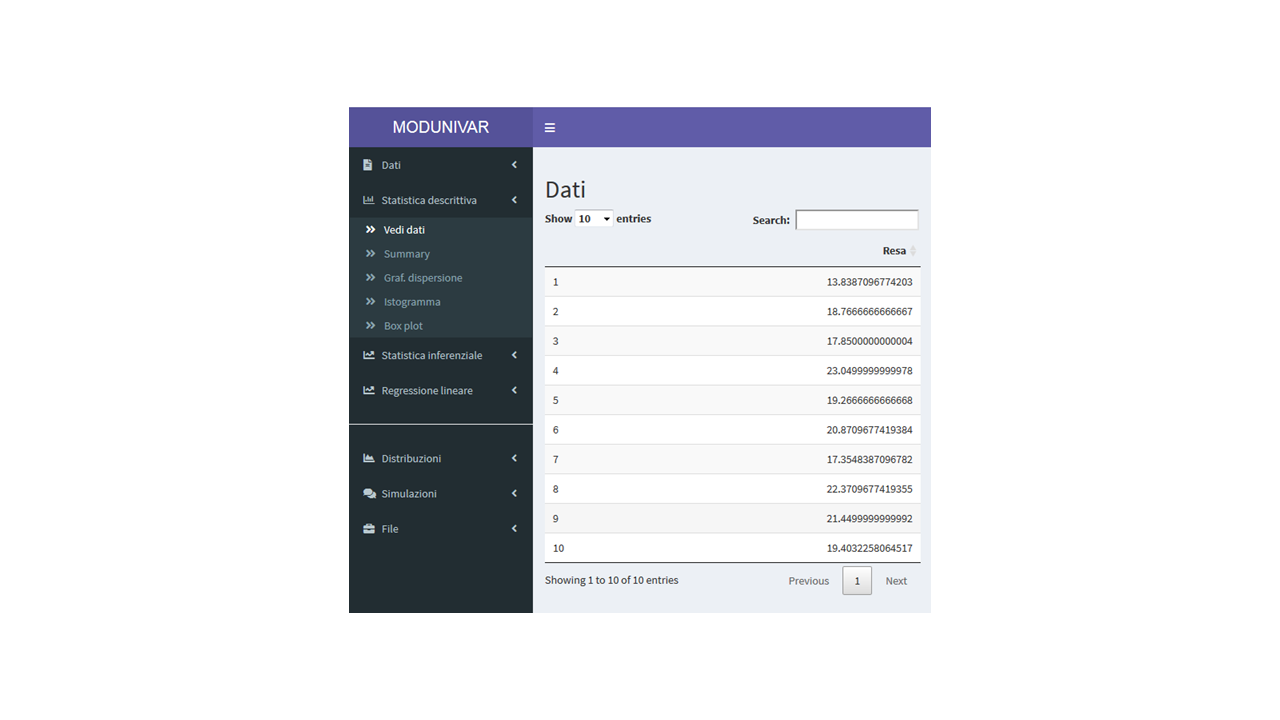
\includegraphics[width=1\linewidth]{Immagini/Descrittiva/2_TabelladatiResa estrattiva} 

}

\caption{Il dataset Resa estrattiva rappresentato in forma di tabella}\label{fig:sd2}
\end{figure}

L'informazione fornita da dieci numeri presentati in forma di elenco però può non essere molto utile, e pertanto spesso si preferisce presentare sia i valori grezzi in forma analitica sia i descrittori di posizione e dispersione dello stesso gruppo di dati. Selezionando la voce ``Summary'' dal menu ``Statistica descrittiva'', la funzione produce la stampa di media aritmetica (mean), deviazione standard (sd), intervallo interquartile (Inter-Quartile Range, IQR, differenza tra il terzo e il primo quartile, v. Glossario), valore minimo della serie (0\%), valore al primo quartile (25\%), mediana (50\%, secondo quartile), valore al terzo quartile (75\%), massimo (100\%) e numero di dati su cui si calcola la statistica.

\begin{figure}

{\centering 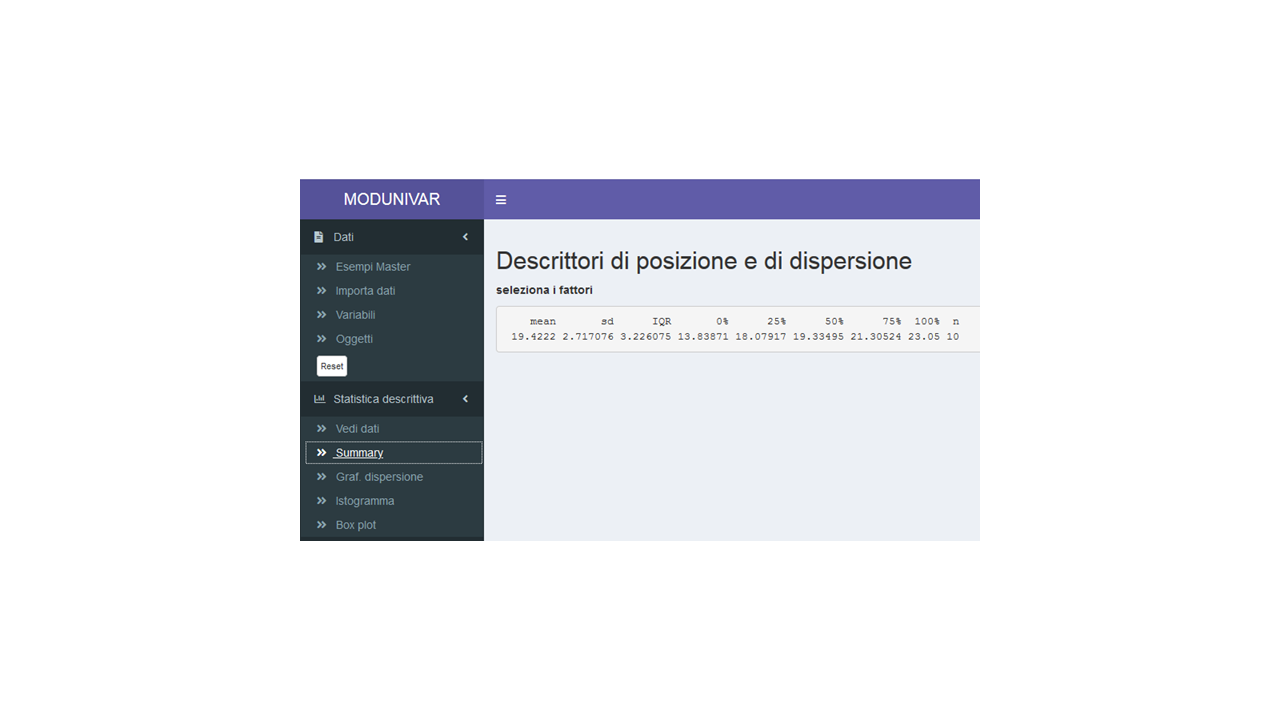
\includegraphics[width=1\linewidth]{Immagini/Descrittiva/3_SummaryResa_estrattiva} 

}

\caption{Indicatori di posizione e dispersione calcolabili dal dataset Resa estrattiva}\label{fig:sd3}
\end{figure}

Il primo strumento grafico di immediata comprensione si ottiene con il comando ``Graf. dispersione'' che stampa il grafico a punti cosiddetto ``a dispersione'', per visualizzare i dati così come sono.
Nel grafico, le rese estrattive si leggono sulle ordinate, mentre in ascissa compare il numero di ordinamento dei dati. La linea blu orizzontale indica il valore della media.

\begin{figure}

{\centering 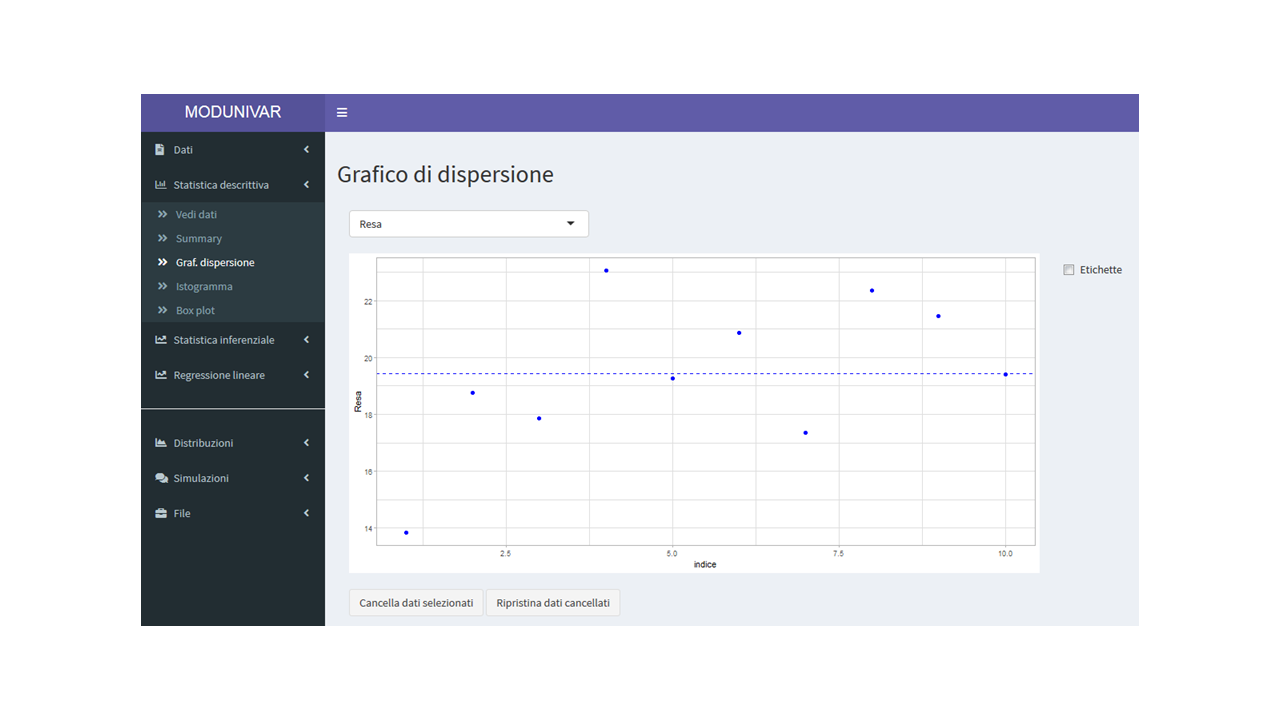
\includegraphics[width=1\linewidth]{Immagini/Descrittiva/4_Graf_dispers Resa_estrattiva} 

}

\caption{Grafico di dispersione dei dati di Resa estrattiva}\label{fig:sd4}
\end{figure}

Il grafico a punti può essere modificato introducendo le ``etichette dei dati'' che, in questo caso, coincidono con il numero di ordinamento dei dati.

Nelle relazioni con dati, è molto frequente incontrare grafici a barre, chiamati Istogrammi. Per ottenere una rappresentazione dei dati del dataset in forma di istogramma è sufficiente selezionare la voce ``Istogramma'' del menu ``Statistica descrittiva''. L'istogramma è un grafico in cui in ordinata sono riportate le rese raggruppate in intervalli definiti attrverso il comando ``larghezza barra''. In ordinata invece è possibile scegliere la forma dei dati da riportare tra tre possibilità: il conteggio dei dati che cadono negli intervalli di resa identificati attraverso il comando ``larghezza barra'', la percentuale del numero di questi dati sul totale dei dati raccolti (percentuale = 100·numero di dati che cadono nell'intervallo dato/10) e la loro densità (densità = area della barra = percentuale/100).

\begin{figure}

{\centering 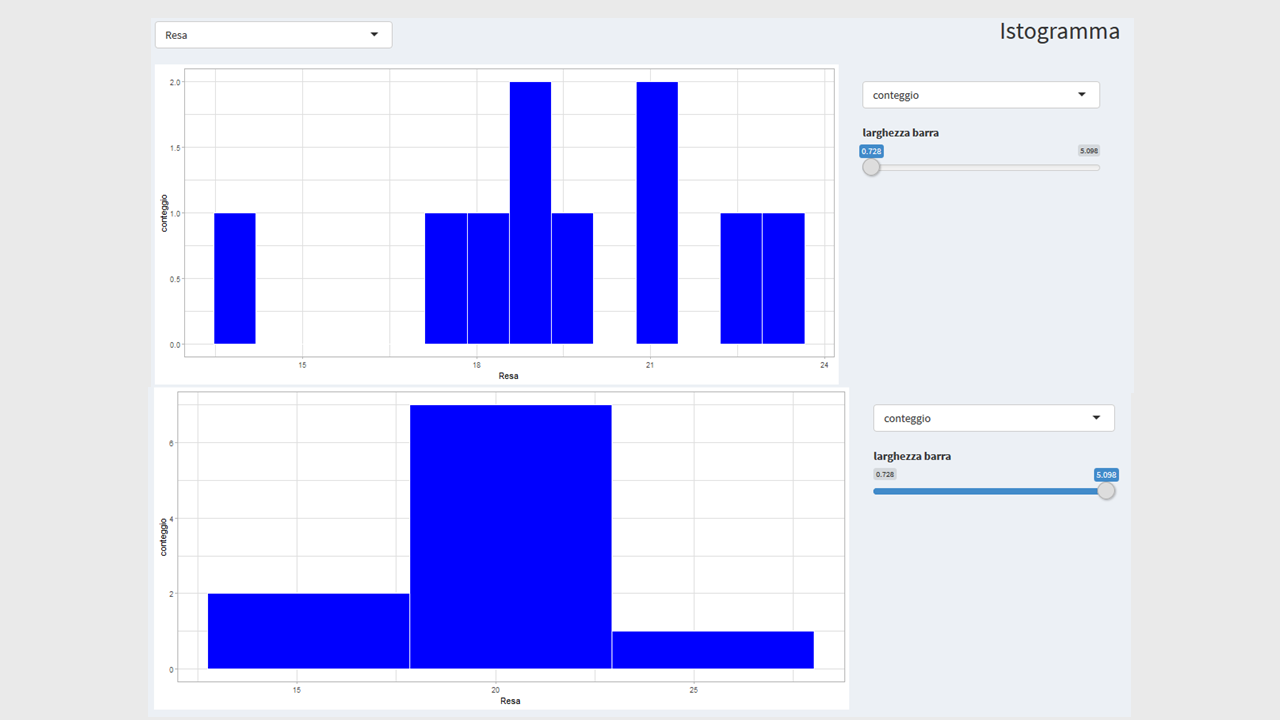
\includegraphics[width=1\linewidth]{Immagini/Descrittiva/5_IstogResaestrattiva} 

}

\caption{Istogrammi dei dati di Resa estrattiva. In alto, la larghezza delle barre è la minima possibile; in basso la larghezza delle barre è la massima possibile}\label{fig:sd5}
\end{figure}

Un altro importante strumento grafico è il ``box-and-whiskers plot'' (o boxplot), che si ottiene usando la funzione Box plot del menu ``Statistica descrittiva''. Il boxplot rappresenta in modo compatto in un unico grafico i maggiori descrittori dei dati.

\begin{figure}

{\centering 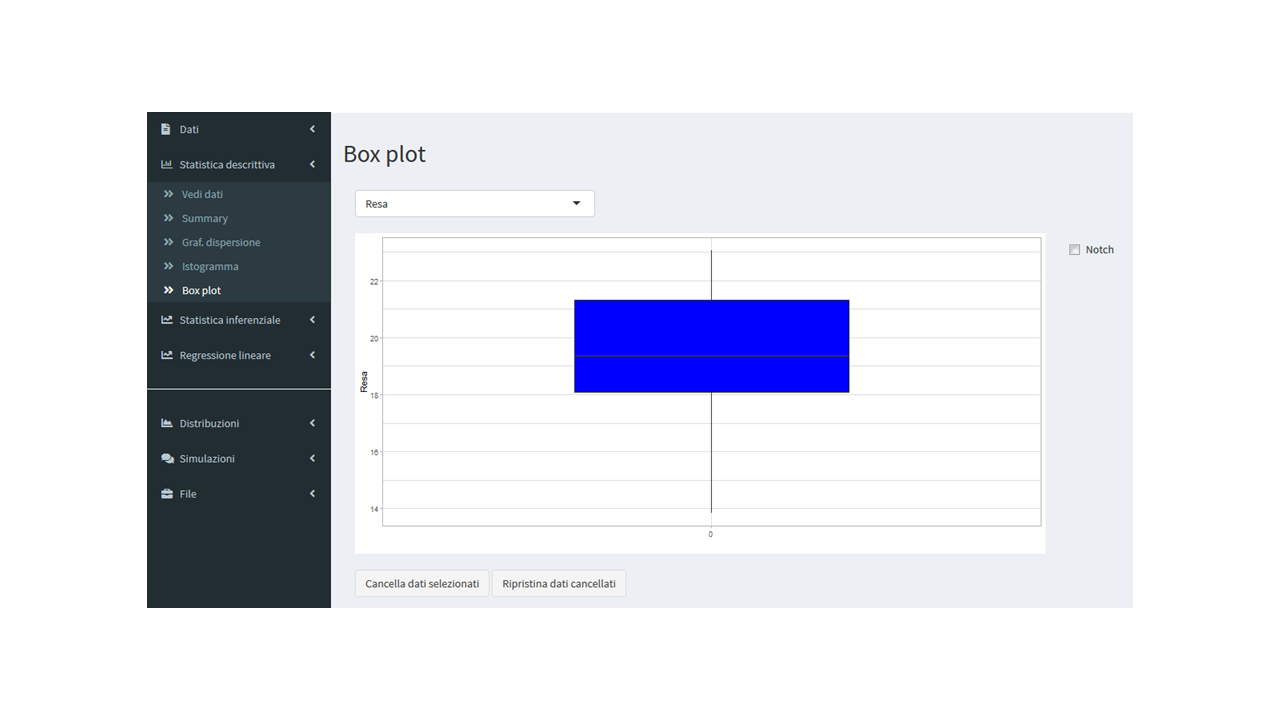
\includegraphics[width=1\linewidth]{Immagini/Descrittiva/6_BoxplotRestrattiva} 

}

\caption{Boxplot dei dati di Resa estrattiva}\label{fig:sd6}
\end{figure}

In ascissa compare un numero di ordine della serie di dati (in questo abbiamo una unica serie e viene assegnato di default il valore ``0'' in ascissa), mentre in ordinata sono riportati i valori di resa etrattiva. La ``scatola'' si estende dal primo al terzo quartile, la riga centrale rappresenta la mediana e i baffi vanno dal valore minimo al valore massimo. I baffi permettono anche di identificare valori anomali (dati aberranti, outliers). Una convenzione grafica accettata è che i dati che cadono fuori dalla scatola ad una distanza di almeno 1.5 volte la dimensione della scatola siano da considerare con sospetto e siano soggetti a verifica con opportuni test per gli outliers (test di Dixon, Grubbs, Cochran o altri).
Si osservi che il valore 1.5 è definito in automatico arbitrariamente dalla routine e nei software di statistica ``aperti'' può essere modificato.

\hypertarget{statistica-inferenziale}{%
\chapter{Statistica inferenziale}\label{statistica-inferenziale}}

\hypertarget{stime-della-media}{%
\section{Stime della media}\label{stime-della-media}}

\hypertarget{una-popolazione-gaussiana}{%
\subsection{Una popolazione gaussiana}\label{una-popolazione-gaussiana}}

Riconsideriamo il dataset \emph{Resa estrattiva} già visto nella parte di Statistica descrittiva:

\begin{verbatim}
##     Resa
## 1  13.84
## 2  18.77
## 3  17.85
## 4  23.05
## 5  19.27
## 6  20.87
## 7  17.35
## 8  22.37
## 9  21.45
## 10 19.40
\end{verbatim}

A differenza del caso precedente, in cui le 10 misure formavano l'intera popolazione in esame, il dataset rappresenta un campione (aleatorio) della popolazione di tutte le misure teoricamente possibili.

Siamo interessati ad ottenere informazioni su tutta la popolazione partendo dal campione (aleatorio) del risultato di
10 misure sperimentali. Ad esempio possiamo chiederci qual' è la media ``vera'' della nostra resa estrattiva o meglio come possiamo stimare tale valore a partire dai 10 risultati sperimentali.

Per fare ciò abbiamo bisogno di conoscere a priori la probabilità di distribuzione di ogni misura.\\
Possiamo supporre che ogni misura sia data dalla media ``vera'' \(\mu\) della nostra resa estrattiva più un errore sperimentale \(\epsilon\) puramente casuale:
\[
y=\mu+\epsilon
\]
L'errore sperimentale \(\epsilon\) può essere supposto distribuito come una normale di media \(0\) e varianza \(\sigma^2\)
\[
\epsilon \sim N(0,\sigma^2)
\]
grazie ad un teorema fondamentale di calcolo delle probabilità (il \emph{teorema centrale del limite}) che dimostra la verità di questa affermazione. Questo teorema afferma che la somma di variabili casuali aventi la stessa distribuzione di probabilità tende ad essere distribuita come una normale indipendentemente dalla loro distribuzione.

Ciò significa che il risultato di una singola misura (che è un valore casuale, dipendente dal campione) può assumere ad esempio i valori come nelle seguenti figure

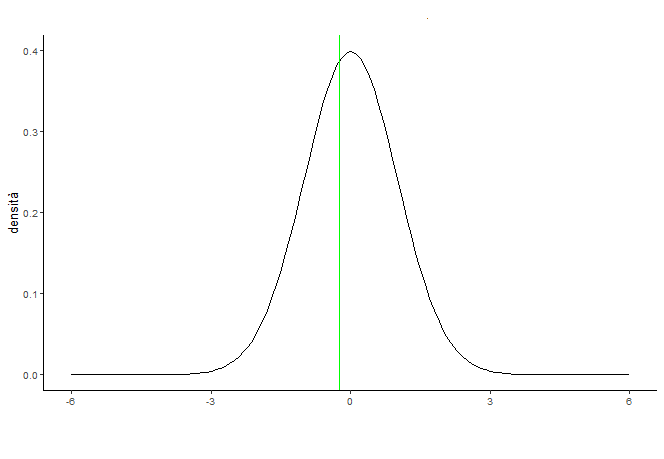
\includegraphics[width=0.35\linewidth]{Immagini/Inferenziale/misura1}
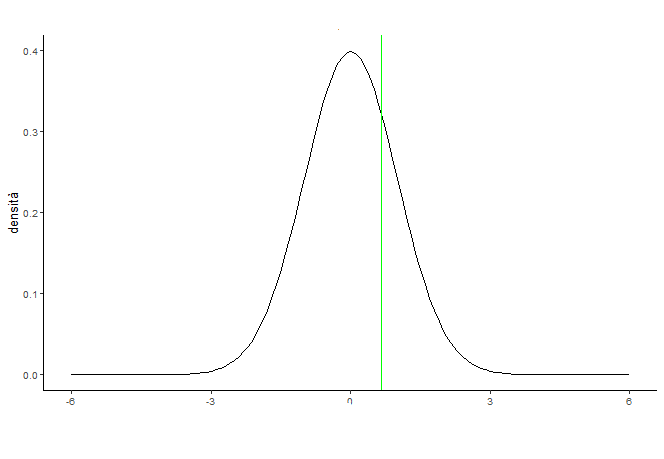
\includegraphics[width=0.35\linewidth]{Immagini/Inferenziale/misura2}
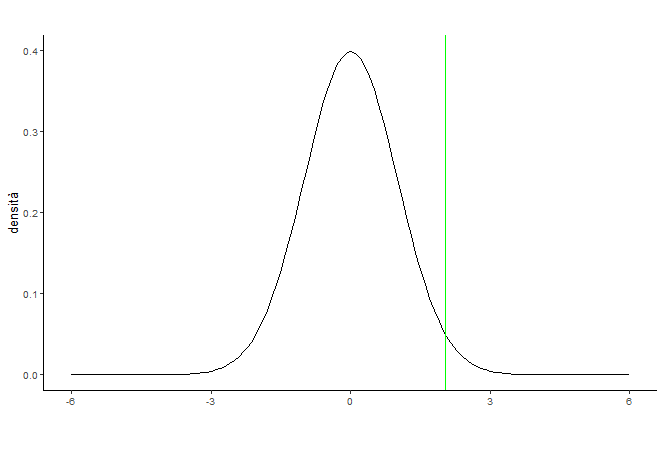
\includegraphics[width=0.35\linewidth]{Immagini/Inferenziale/misura3}

ma certamente sappiamo (sapendo che la sua distribuzione è una normale), ad esempio, che il risultato della misura sarà nella zona bianca della figura seguente con una probabilità pari al 95\%

\begin{center}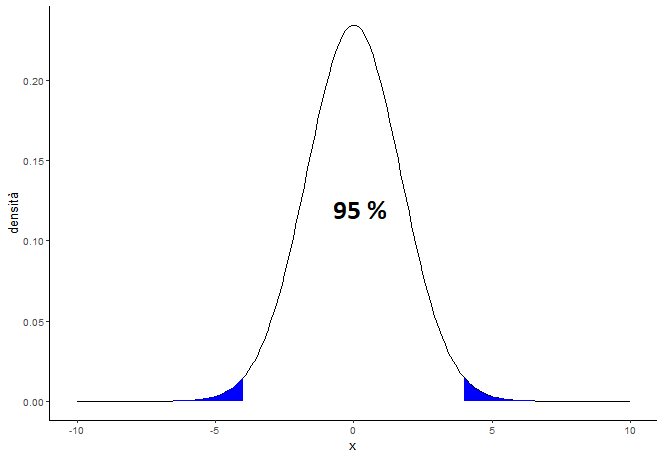
\includegraphics[width=0.5\linewidth]{Immagini/Inferenziale/probamis} \end{center}

Altra importante ipotesi è che le misure siano indipendenti le une dalle altre, ossia che il risultato di ogni misura non sia influenzato in alcun modo da una misura precedente.

Osservazione: alla luce di quanto sopra, come devono essere eseguiti gli esperimenti, ad esempio nella costruzione di una curva di taratura?
E' corretta la prassi di predisporre i calibratori in ordine crescente di concentrazione?

Riassumendo: a partire dal risultato di \(10\) misure distribuite come una normale di media \(\mu\) e varianza \(\sigma^2\)
\[
y_i=\mu+\epsilon_i, \qquad \epsilon_i \sim N(0,\sigma^2)
\]
supponiamo che le misure siano tutte indipendenti tra loro e quindi ci poniamo il problema della stima della media ``vera'' della nostra resa estrattiva, ossia del parametro \(\mu\).

Si noti che grazie al \emph{teorema centrale del limite} è possibile alleggerire le ipotesi nel caso in cui il numero \(m\) di osservazioni (la numerosità del campione) è grande, ad esempio \(m>30\). In tal caso è sufficiente supporre che le misure siano identicamente distribuite (cioè che abbiano la stessa distribuzione di probabilità, non importa quale) e indipendenti tra loro.

\hypertarget{varianza-sigma2-nota}{%
\subsubsection{\texorpdfstring{Varianza \(\sigma^2\) nota}{Varianza \textbackslash sigma\^{}2 nota}}\label{varianza-sigma2-nota}}

In questo paragrafo supponiamo che la varianza \(\sigma^2\) della popolazione sia nota a priori; nel paragrafo successivo ci occuperemo del caso (più frequente) in cui \(\sigma^2\) non sia nota e dunque debba essere stimata.

A partire dal risultato delle \(10\) misure sperimentali del nostro campione possiamo considerare la variabile \(\bar{y}\), definita come la ``media'' delle \(10\) misure
\[
\bar{y}=\frac{\sum_{i=1}^{10}y_i}{10}
\]
La variabile \(\bar{y}\) è una variabile casuale (dipende dal campione di \(10\) misure che è estratto in modo casuale dalla popolazione) ma, grazie alle proprietà della distribuzione normale delle \(y_i\) e all'ipotesi di indipendenza delle misure, è facile dimostare che essa - la media delle misure- è distribuita come una normale di media \(\mu\) e varianza \(\sigma^2/10\)
\[
\bar{y}\sim N(\mu,\sigma^2/10)
\]
La quantità \(\sigma/\sqrt{10}\) è chiamata \emph{errore standard della media}
(Attenzione! da non confondere con la deviazione standard dalla media)

\begin{center}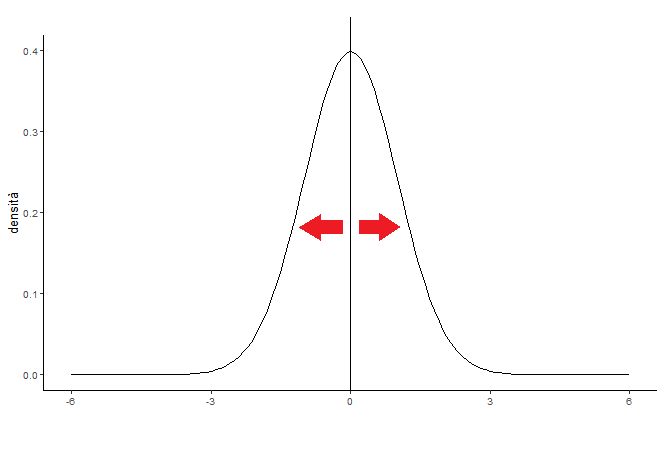
\includegraphics[width=0.5\linewidth]{Immagini/Inferenziale/varianza_media} \end{center}

ed è un indicatore della variazione della stima puntuale \(\bar{y}\) della media \(\mu\) (proprietà che chiamiamo ``precisione'' della stima e che coincide con la qualità della stima stessa; una stima di ``buona'' qualità è un dato che ha piccolo errore standard ossia alta precisione).
L'\emph{errore standard della media} \(\sigma/\sqrt{m}\) diminuisce all'aumentare della numerosità \(m\) del campione. Per aumentare la precisione occorre quindi aumentare il numero di campioni (nel nostro esempio la precisione della stima con \(m=10\) può essere migliorata se aumentiamo m, il numero dei campioni, per fissare le idee poniamo \(m=20\)).

\hypertarget{intervallo-di-confidenza}{%
\paragraph{Intervallo di confidenza}\label{intervallo-di-confidenza}}

La stima puntuale \(\bar{y}\) del parametro \(\mu\) è una risposta piuttosto grossolana al problema di determinare una buona approssimazione del valore vero incognito.
In particolare ricordiamo che il valore stimato sperimentalmente non sarà mai uguale al valore vero (per di più, per definizione, il valore vero non è nemmeno noto\ldots).

Vediamo quindi come possiamo determinare una stima per intervalli del parametro \(\mu\): cerchiamo di definire il cosiddetto ``intervallo di confidenza''.

Grazie alle note proprietà della normale si può dimostrare che:

\[
\bar{y}-\mu \sim N(0,\sigma^2/10)
\]
e che

\[
\frac{\bar{y}-\mu}{\sigma\sqrt{1/10}} \sim N(0,1)
\]

Riassumendo: a partire dal risultato delle \(10\) misure abbiamo calcolato la variabile \(\frac{\bar{y}-\mu}{\sigma\sqrt{1/10}}\). Essa è una variabile casuale (dipende dal campione di \(10\) misure che è stato estratto in modo casuale dalla popolazione) di cui conosciamo la distribuzione di probabilità.

Nel menù Simulazione /Stima della media del programma è possibile simulare quanto detto. Supponiamo che la media della popolazione
(che a priori non conosciamo) sia \(\mu=19\), che la deviazione standard sia \(\sigma=2.7\) e che la numerosità del campione sia \(m=10\)

\begin{center}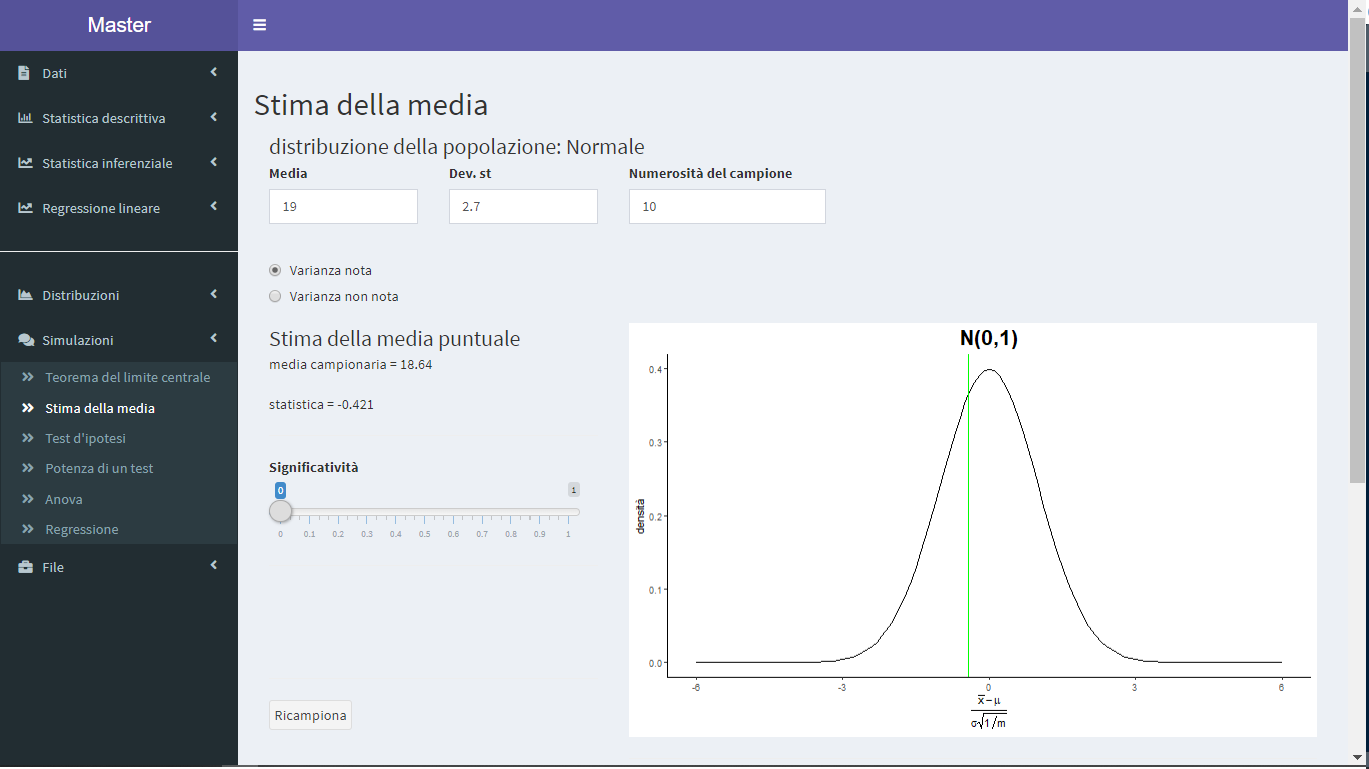
\includegraphics[width=0.5\linewidth]{Immagini/Inferenziale/simulazione_media} \end{center}

cliccando sul bottone \emph{Ricampiona} si simula il risultato \(\frac{\bar{y}-\mu}{\sigma\sqrt{1/10}}\) ottenuto da \(10\) nuove misure sperimentali (cioè da un nuovo campione casuale di numerosità \(10\) della popolazione in esame)

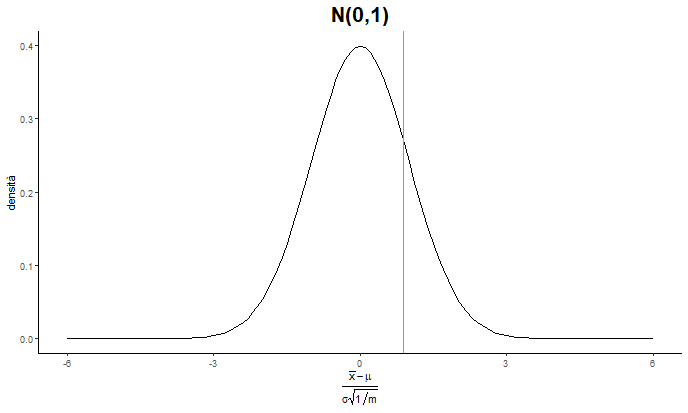
\includegraphics[width=0.35\linewidth]{Immagini/Inferenziale/simulazione_media1}
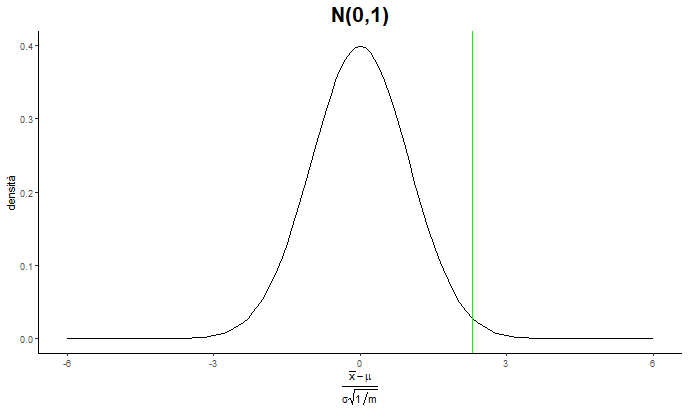
\includegraphics[width=0.35\linewidth]{Immagini/Inferenziale/simulazione_media2}
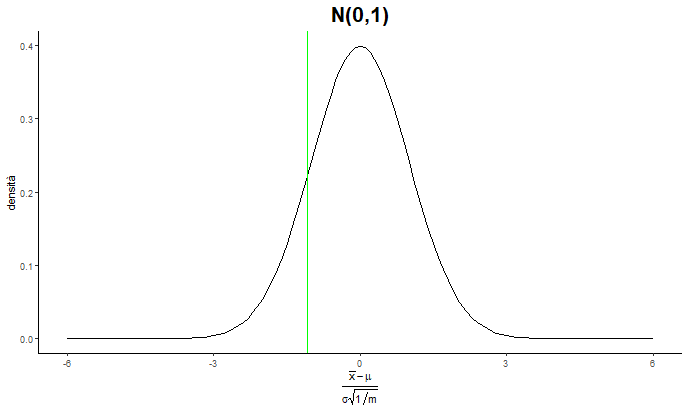
\includegraphics[width=0.35\linewidth]{Immagini/Inferenziale/simulazione_media3}

Fissando la significatività ad esempio a \(0.05\) si ha che \(\frac{\bar{y}-\mu}{\sigma\sqrt{1/10}}\) ha il \(95\)\% di probabilità di assumere valori (la linea verde) nella regione bianca, come ad esempio in figura

\begin{center}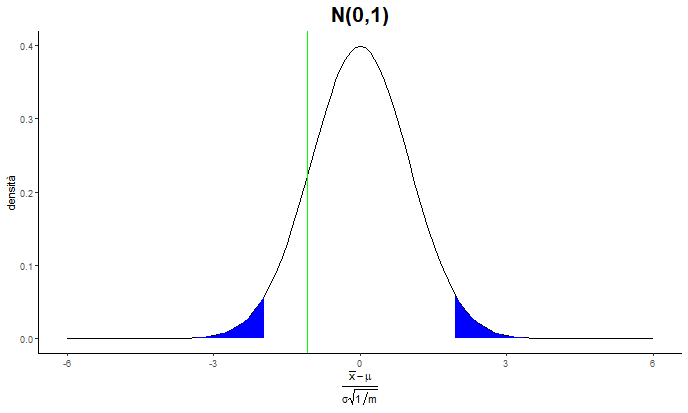
\includegraphics[width=0.5\linewidth]{Immagini/Inferenziale/simulazione_media4} \end{center}

Riprendiamo la costruzione dell'intervallo di confidenza. Fissiamo un valore \(\alpha\) compreso tra \(0\) e \(1\) (in generale si fissa \(\alpha=0.05\)). Indichiamo con \(z_{\alpha/2}\) il quantile di ordine \(1-\alpha/2\) della distribuzione normale \(N(0,1)\), ossia quel numero reale per cui una variabile \(z\) casuale distribuita come \(N(0,1)\) abbia probablità \(1-\alpha/2\) di assumere valore minore di \(z_{\alpha/2}\)
\[
\mathbb{P}[z < z_{\alpha/2}] = 1-\alpha/2
\]

In particolare, essendo \(\frac{\bar{y}-\mu}{\sigma\sqrt{1/10}} \sim N(0,1)\), avremmo che

\[
\mathbb{P}[\frac{\bar{y}-\mu}{\sigma\sqrt{1/10}} < z_{\alpha/2}] = 1-\alpha/2
\]

Nell'esempio del simulatore, \(z_{\alpha/2}\) indica il valore sulle ascisse di confine destro tra la zona blu e la zona bianca.

Abbiamo quindi

\[
\mathbb{P}[- z_{\alpha/2}<\frac{\bar{y}-\mu}{\sigma\sqrt{1/10}} < z_{\alpha/2}] = 1-\alpha
\]

che, sempre nell'esempio del simulatore, è la probabilità che la linea verde cada nella zona bianca (vedi figura sopra).

Possiamo quindi costruire il seguente \emph{intervallo di confidenza di livello \(\alpha\)}
\[
\bar{y} \pm z_{\alpha/2} \sigma \sqrt{1/10}
\]
Questo un intervallo aleatorio, perché dipende dal campione di \(10\) misure (estratto in modo casuale dalla popolazione). Nel simulatore, infatti, se clicchiamo sul bottone \emph{Ricampiona} otteniamo intervalli diversi.

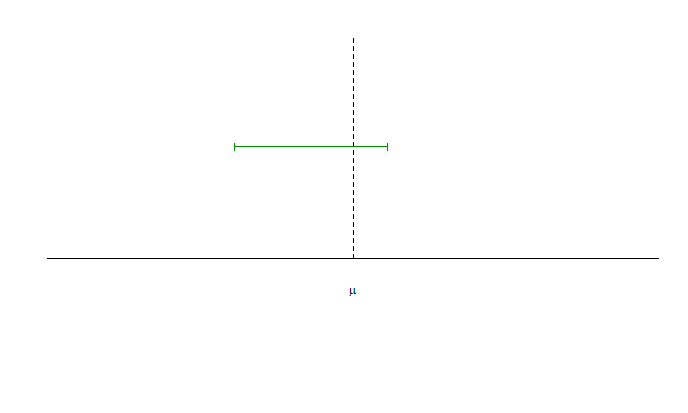
\includegraphics[width=0.35\linewidth]{Immagini/Inferenziale/intconf1}
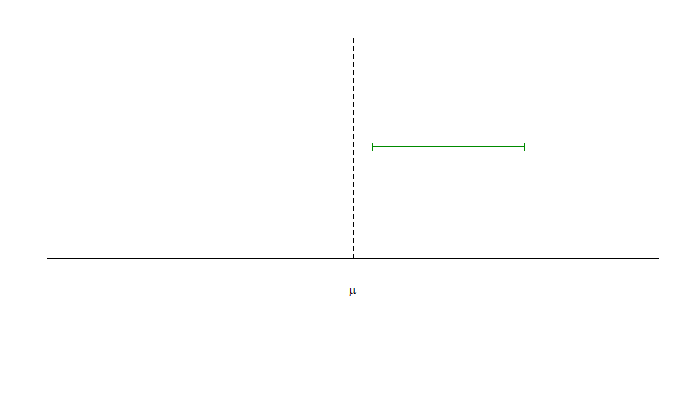
\includegraphics[width=0.35\linewidth]{Immagini/Inferenziale/intconf2}
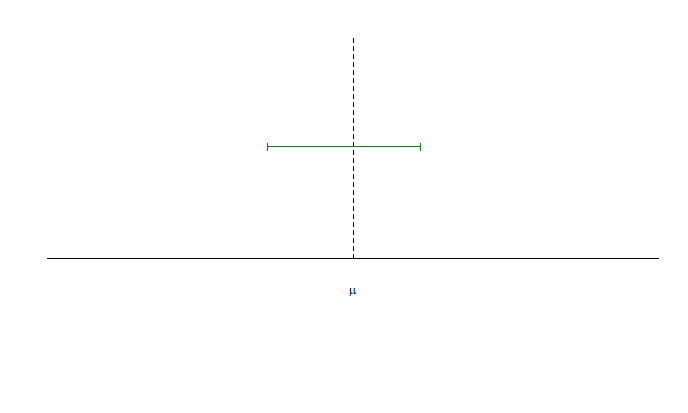
\includegraphics[width=0.35\linewidth]{Immagini/Inferenziale/intconf3}

L'\emph{intervallo di confidenza di livello \(\alpha\)} ha come caratteristica questa proprietà. Ripetendo un numero elevato di volte la costruzione dell'intervallo a partire da un nuovo campione (\(10\) nuove misure sperimentali) circa \(1-\alpha\) di questi intervalli contiene il valore \(\mu\).
Nel simulatore, cliccando un numero elevato di volte il bottone \emph{Ricampiona}, circa il \(95\%\) degli intervalli costruiti conterrà la linea tratteggiata verticale (valore di \(\mu\))

\hypertarget{test-di-ipotesi}{%
\paragraph{Test di ipotesi}\label{test-di-ipotesi}}

A partire da quanto detto è possibile anche fare il seguente test di ipotesi sulla media:
\[
 H_0: \mu=\mu_0 \quad \rm{vs} \quad H_1: \mu \neq \mu_0 \quad 
\]
cioè supponiamo che la media ``vera'' \(\mu\) sia uguale ad un certo valore \(\mu_0\) e vediamo se le informazioni ricavabili dal nostro campione di \(10\) misure sono tali da portarci a confutare questa ipotesi.
La procedura di esecuzione di un test di ipotesi è sempre la stessa ed inizia formulando la affermazione seguente: consideriamo l'ipotesi \(\mu=\mu_0\) vera fino ``a prova contraria''.

Fissato un valore \(\alpha\) per quanto sopra detto, nell'ipotesi \(\mu=\mu_0\), abbiamo che

\[
\mathbb{P}[- z_{\alpha/2}<\frac{\bar{y}-\mu_0}{\sigma\sqrt{1/10}} < z_{\alpha/2}] = 1-\alpha
\]

Ad esempio nel menù Simulazioni/Test d'ipotesi, ragionando come sopra,

\begin{center}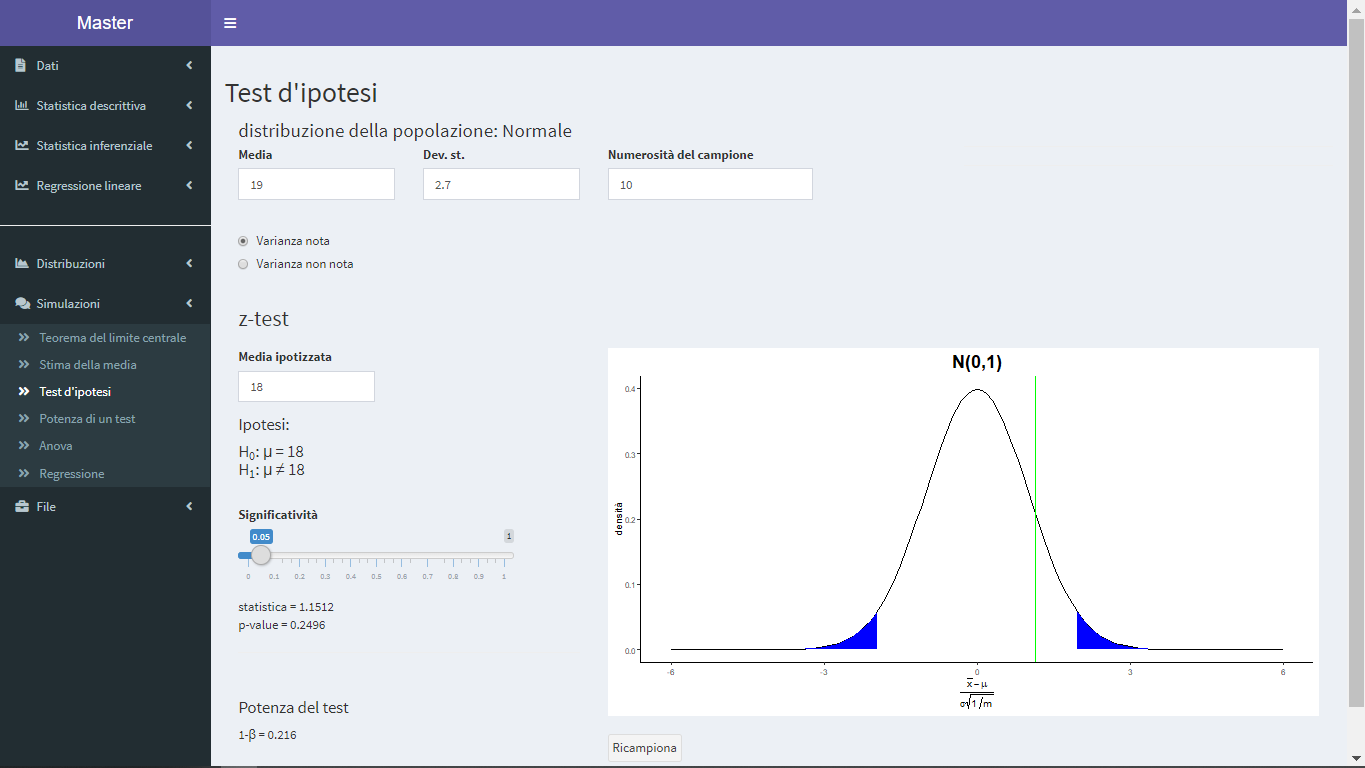
\includegraphics[width=0.5\linewidth]{Immagini/Inferenziale/test_ip} \end{center}

supponendo \(\mu=18\), cliccando sul bottone \emph{Ricampiona} si simula il risultato \(\frac{\bar{y}-\mu_0}{\sigma\sqrt{1/10}}\) ottenuto da \(10\) nuove misure sperimentali (cioè da un nuovo campione casuale di numerosità \(10\) della popolazione in esame)

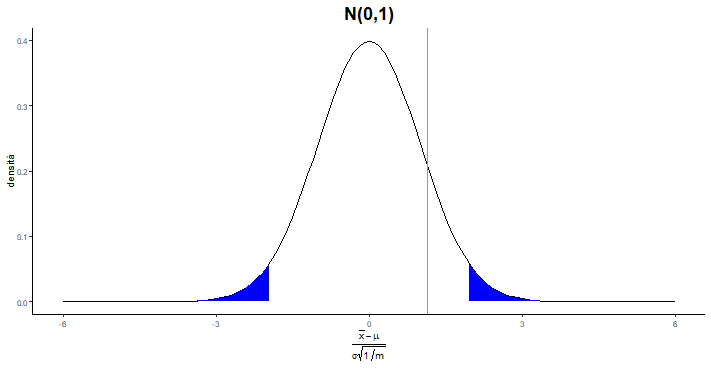
\includegraphics[width=0.35\linewidth]{Immagini/Inferenziale/test_ip1}
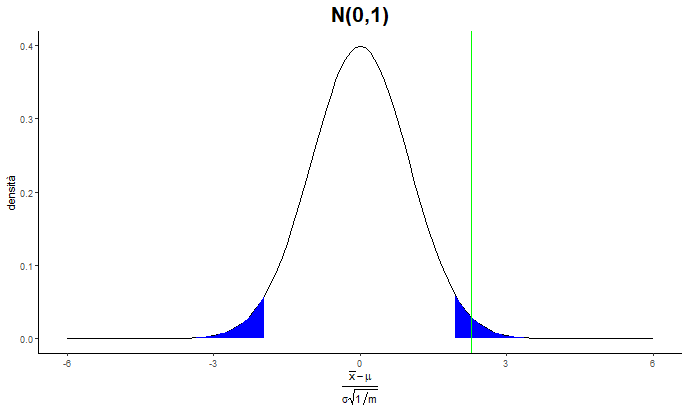
\includegraphics[width=0.35\linewidth]{Immagini/Inferenziale/test_ip2}
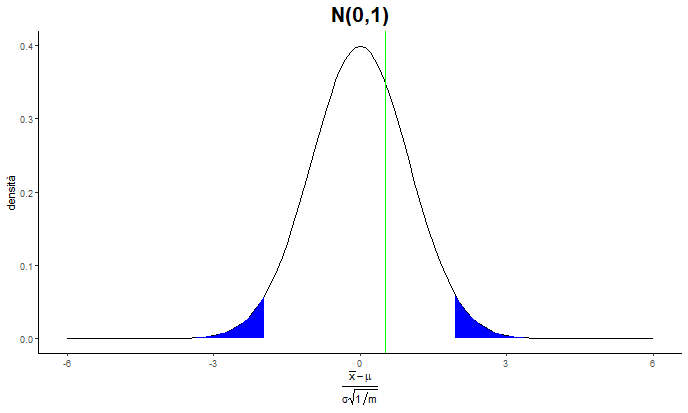
\includegraphics[width=0.35\linewidth]{Immagini/Inferenziale/test_ip3}

Siccome noi supponiamo vera l'ipotesi nulla \(H_0\), il \(95 \%\) (\(\alpha=0.05\)) delle volte il valore \(\frac{\bar{y}-\mu_0}{\sigma\sqrt{1/10}}\) deve cadere nella zona bianca mentre il restante \(5 \%\) cade nella zona blu \emph{Regione Critica}.

Accettiamo l'ipotesi nulla \(H_0\) se la stima \(\frac{\bar{y}-\mu_0}{\sigma\sqrt{1/10}}\) non cade nella \emph{Regione Critica} (primo e terzo caso caso nella figura precedente) infatti, in tal caso non abbiamo evidenza statistica per rifiutare l'ipotesi nulla, mentre rifiutiamo l'ipotesi nulla nel caso contrario (secondo caso figura precedente).
In tal caso diremo che \(\mu\) è diversa da \(\mu_0\) al livello di significatività \(\alpha\) (o che \(\mu\) è significativamente diversa da \(\mu_0\) al livello \(\alpha\)).
Si osservi che \(\alpha\) è la probabilità di rifiutare l'ipotesi nulla \(H_0\) quando questa è vera (errore di tipo I) e, ovviamente, si vuole che tale probabilità sia piccola.

Per eseguire il test nell'esempio \emph{Resa estrattiva} si procede come segue: si carica il dataset nel menù Statistica inferenziale/Test media. Si sceglie il caso di una popolazione, si indica il valore della deviazione standard nota (N.B. stiamo supponendo che \(\sigma\) sia nota a priori), ad esempio \(\sigma =2.7\) e si indica infine la media ipotizzata, ad esempio \(\mu_0=18\). Quindi si fissa la significatività \(\alpha\), ad esempio \(\alpha=0.05\). Abbiamo evidenza statistica per rifiutare \(H_0\) se la linea verde (che indica il valore \(\frac{\bar{y}-\mu_0}{\sigma\sqrt{1/10}}\) calcolato dal nostro campione) è nella \emph{Regione Critica}, ossia cade nella regione blu. In caso contrario accettiamo \(H_0\) non avendo evidenza statistica per rifiutarla.
Attenzione! Non abbiamo provato che \(H_0\) è \emph{vera} (ipotesi a priori). Il responso del test di ipotesi è che le informazioni contenute nel nostro campione (la media e la deviazione standard) non sono tali da fornire prove sufficienti per rifiutarla e dire quindi che la media del campione è diversa da quella della popolazione al livello di significatività \(\alpha=0.05\).

Un importante indicatore di un test d'ipotesi è il \emph{p-value}. E' la probabilità che una variabile aleatoria distribuita come la \(N(0,1)\) assuma valori (in valore assoluto) maggiori di \(\frac{\bar{y}-\mu_0}{\sigma\sqrt{1/10}}\)

\[
\mathbb{P}[|z|>|\frac{\bar{y}-\mu_0}{\sigma\sqrt{1/10}}|], \qquad z \sim N(0,1)
\]

Il \emph{p-value} è il più piccolo valore di \(\alpha\) per cui abbiamo evidenza statistica per rifiutare \(H_0\). E il ``vero'' livello di significatività per cui rifiutiamo \(H_0\).

Accettiamo \(H_0\) se il \emph{p-value} è maggiore di \(\alpha\) (immagine a destra nella figura sottostante) e rifiutiamo \(H_0\) nel caso contario (immagine a sinistra nella figura sottostante)

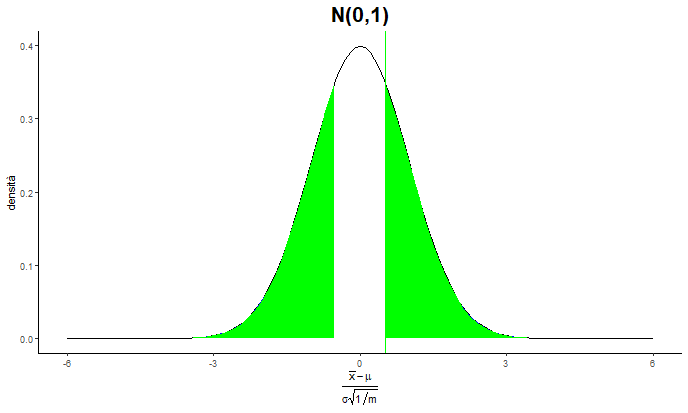
\includegraphics[width=0.5\linewidth]{Immagini/Inferenziale/pval}
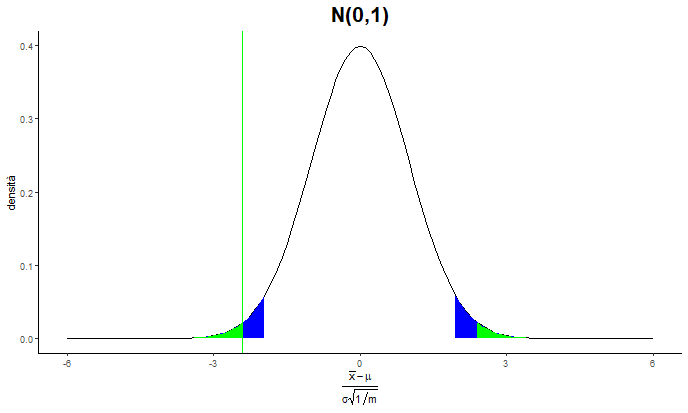
\includegraphics[width=0.5\linewidth]{Immagini/Inferenziale/pval1}

Ragionando con l'\emph{intervallo di confidenza}, accettiamo \(H_0\) se \(\mu_0\) appartiene all'intervallo, in caso contrario rifiutiamo \(H_0\).

Il valore del \emph{p-value} e gli estremi dell'\emph{intervallo di confidenza}, così come il valore della statistica \(\frac{\bar{y}-\mu_0}{\sigma\sqrt{1/10}}\), si ottengono nel menù Statistica inferenziale/Test media: una popolazione

\begin{center}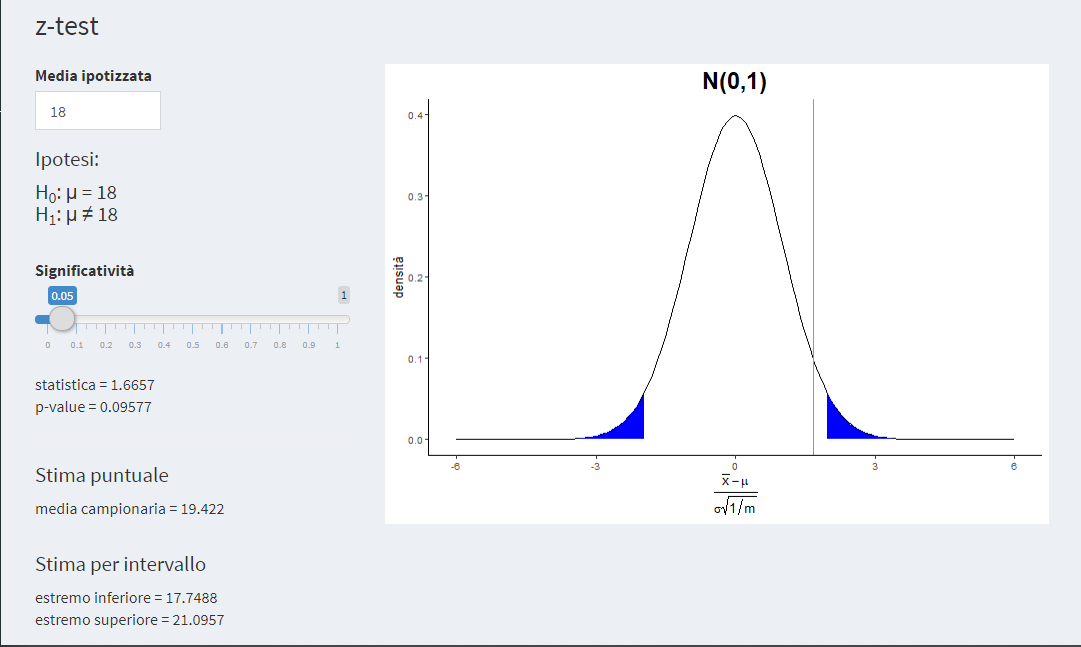
\includegraphics[width=0.5\linewidth]{Immagini/Inferenziale/test_ip4} \end{center}

\hypertarget{verifica-delle-ipotesi}{%
\subsubsection{Verifica delle ipotesi}\label{verifica-delle-ipotesi}}

Dobbiamo verificare che le \(10\) misure sperimentali provengano da una popolazione normale. Questa è l'ipotesi fondamentale da cui siamo partiti affiché tutto ciò detto fin qui sia valido. Ricordiamo che nel caso in cui il campione si sufficientemente grande (ad esempio \(m>30\)) questa ipotesi si può attenuare grazie al \emph{teorema centrale del limite}. In tal caso è sufficiente supporre che le misure siano identicamente distribuite (cioè che abbiano la stessa distribuzione di probabilità, non importa quale).

L'ipotesi di normalità può essere verificata mediante un grafico che riporta in ascissa i quantili della \(N (0 , 1)\) e in ordinate i quantili della distribuzione campionaria dei dati. Tanto più i quantili sono allineati tanto più i dati confermano l'ipotesi di normalità.

Esiste anche un test d'ipotesi specifico, il \emph{test di Shapiro-Wilk}, considerato uno dei più potenti per la verifica della normalità, soprattutto per campioni poco numerosi. Il test confronta una varianza ottenuta usando pesi particolari con la
varianza campionaria. Indicato con \(W\) il rapporto tra le due stime della varianza (\(0 < W < 1\)), nell'ipotesi di
normalità (ipotesi nulla \(H_0\)) si rifiuta l'ipotesi nulla per valori di W troppo piccoli. Il risultato del test è il parametro \(W\) a cui è associato un \emph{p-value}. Il significato rimane quello detto per cui un \emph{p-value} sufficientemente piccolo
(\(p < \alpha\)) è un indice della probabilità che la distribuzione non sia normale.

\begin{center}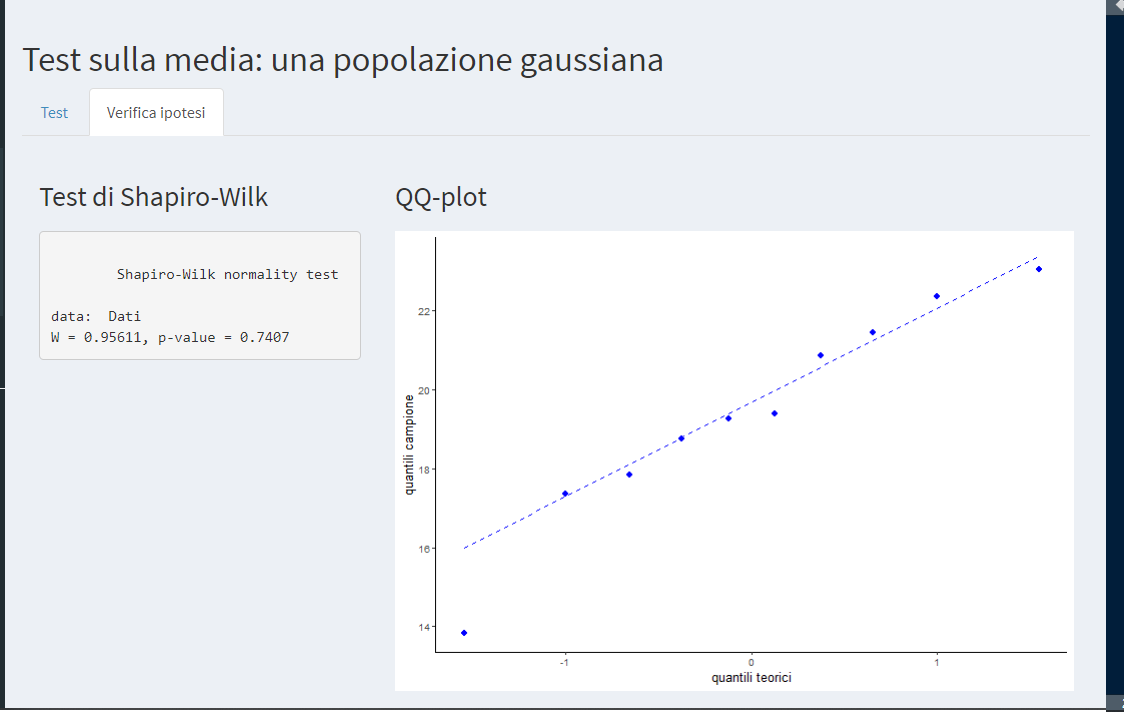
\includegraphics[width=0.5\linewidth]{Immagini/Inferenziale/test_ip_verfipo} \end{center}

La figura rappresenta la verifica di ipotesi eseguita per l'esempio considerato (menù Statistica inferenziale/Test media: una popolazione - pagina Verifica ipotesi)

Quanto illustrato in questo paragrafo in merito ai testi di ipotesi è valido in tutto il capitolo. Per verificare le ipotesi si segue la procedura descritta a partire dalla formulazione della ipotesi nulla, si calcola la statistica del test di interesse (in questo caso, la W di Shapiro-Wilk) e si stabilisce dal valore del parametro stimato se l'ipotesi nulla può essere accettata (\(H_0\): la distribuzione dei dati è normale) o deve essere rifiutata (\(H_1\): la distribuzione non è normale).

\hypertarget{varianza-sigma2-non-nota}{%
\subsubsection{\texorpdfstring{Varianza \(\sigma^2\) non nota}{Varianza \textbackslash sigma\^{}2 non nota}}\label{varianza-sigma2-non-nota}}

In questo caso dobbiamo stimare anche \(\sigma^2\). Una stima puntuale della varianza \(\sigma^2\) è data da
\[
s^2 = \frac{1}{m-1}\sum_{j=1}^m (y_j-\bar y)^2.
\]
(\(m=10\) nel nostro esempio).

Si può quindi dimostrare che
\[
\frac{\bar y - \mu}{s \sqrt{1/m}} \sim t(m-1),
\]
dove \(t(m-1)\) è la distribuzione di Student a \(m-1\) gradi di libertà.

Come si vede dalla figura sottostante la forma della \(t\) di Student dipende dai gradi di libertà e, al crescere di questi ultimi, si ``avvicina'' alla normale \(N(0,1)\). Chiaramente il dover stimare anche \(\sigma\) fa perdere un po' di precisione che ``migliora'' però al crescere della numerosità campionaria.

\begin{center}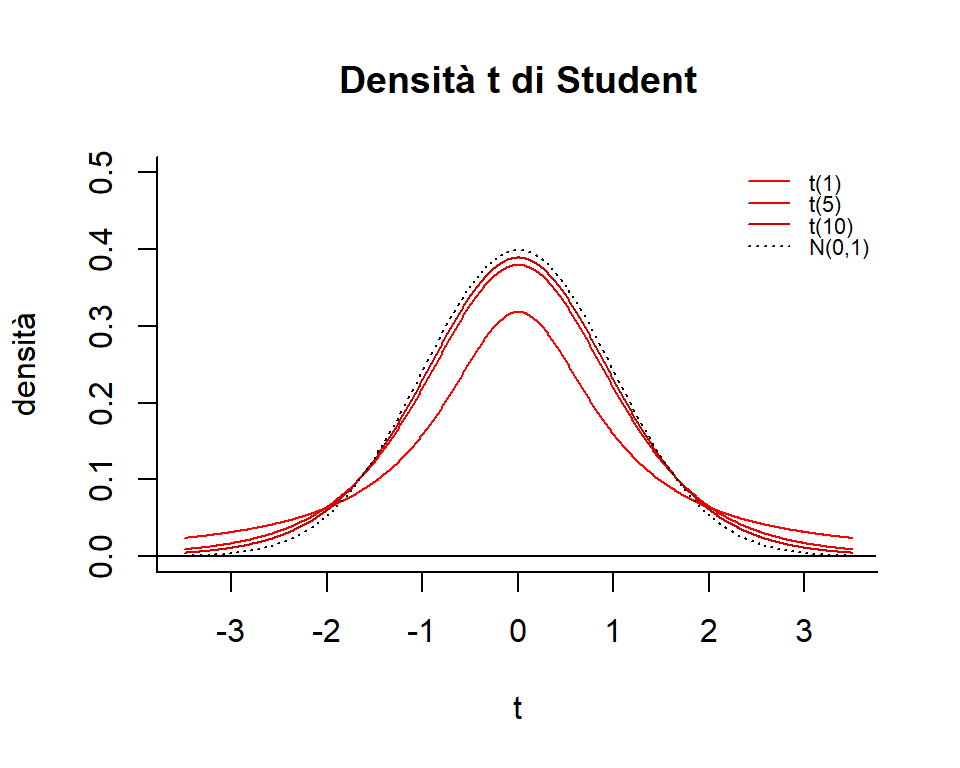
\includegraphics[width=0.5\linewidth]{Immagini/Inferenziale/student} \end{center}

La quantità \(s\) nella formula precedente è la deviazione standard del campione,
è una stima - consistente non distorta - della deviazione standard della popolazione.\\
La quantità \(s \sqrt{1/m}\) è \emph{l'errore standard della media},
ossia la stima della deviazione standard della media.
È dunque una stima della variabilità della stima della media, cioè una misura della sua imprecisione.

Grazie alla conoscenza della distribuzione di probabilità di \(\frac{\bar y - \mu}{s \sqrt{1/m}}\) , possiamo ragionare come nel paragrafo precedente, e fare inferenza per \(\mu\).

Fissiamo un valore \(\alpha\) compreso tra \(0\) e \(1\) (in generale si fissa \(\alpha=0.05\)). Indichiamo con \(t_{\alpha/2}\) il quantile di ordine \(1-\alpha/2\) della distribuzione normale \(t(m-1)\), ossia quel numero reale per cui una variabile \(t\) casuale distribuita come \(t(m-1)\) abbia probablità \(1-\alpha/2\) di assumere valore minore di \(t_{\alpha/2}\)
\[
\mathbb{P}[t < t_{\alpha/2}] = 1-\alpha/2
\]

\begin{itemize}
\item
  \emph{intervallo di confidenza}
  \[
  \bar{y} \pm t_{\alpha/2}s\sqrt{1/m}
  \]
\item
  \emph{test d'ipotesi (t-test)}
  \[
   H_0: \mu=\mu_0 \quad \rm{vs} \quad H_1: \mu \neq \mu_0 \quad 
  \]
\end{itemize}

Come nel caso della varianza nota vanno verificate le ipotesi. Si procede esattamente come quanto visto nel paragrafo precedente.

Tornando al nostro esempio: supponiamo che da un altro gruppo di esperimenti sulla stessa pianta si ottiene il
valore medio di \(18.02\). Vogliamo verificare se possiamo accettare l'ipotesi nulla \(\mu_0=18.02\). Ci chiediamo ``\(18.02\) e \(19.42\) (media campionaria) sono
statisticamente distinguibili''?
(N.B. il fatto che due dati siano \emph{numericamente diversi} non vuole dire che lo siano anche \emph{statisticamente}. Questo è l'oggetto della verifica in questione).
Per eseguire il test si procede come nel caso precedente: una volta caricato il dataset, nel menù Statistica inferenziale/Test media si sceglie il caso di una popolazione e si clicca su \emph{Varianza non nota}, si indica infine la media ipotizzata, ad esempio \(\mu_0=18.02\). Quindi si fissa la significatività \(\alpha\), ad esempio \(\alpha = 0.05\).
Abbiamo evidenza statistica per rifiutare \(H_0\) se la linea verde (che indica il valore \(\frac{\bar{y}-\mu_0}{\sigma\sqrt{1/10}}\) calcolato dal nostro campione) è nella \emph{Regione Critica}, ossia cade nella regione blu. In caso contrario accettiamo \(H_0\) non avendo evidenza statistica per rifiutarla.

Il valore del \emph{p-value} e gli estremi dell'\emph{intervallo di confidenza}, così come il valore della statistica \(\frac{\bar{y}-\mu_0}{\sigma\sqrt{1/10}}\), si ottengono nel menù Statistica inferenziale/Test media: una popolazione

\begin{center}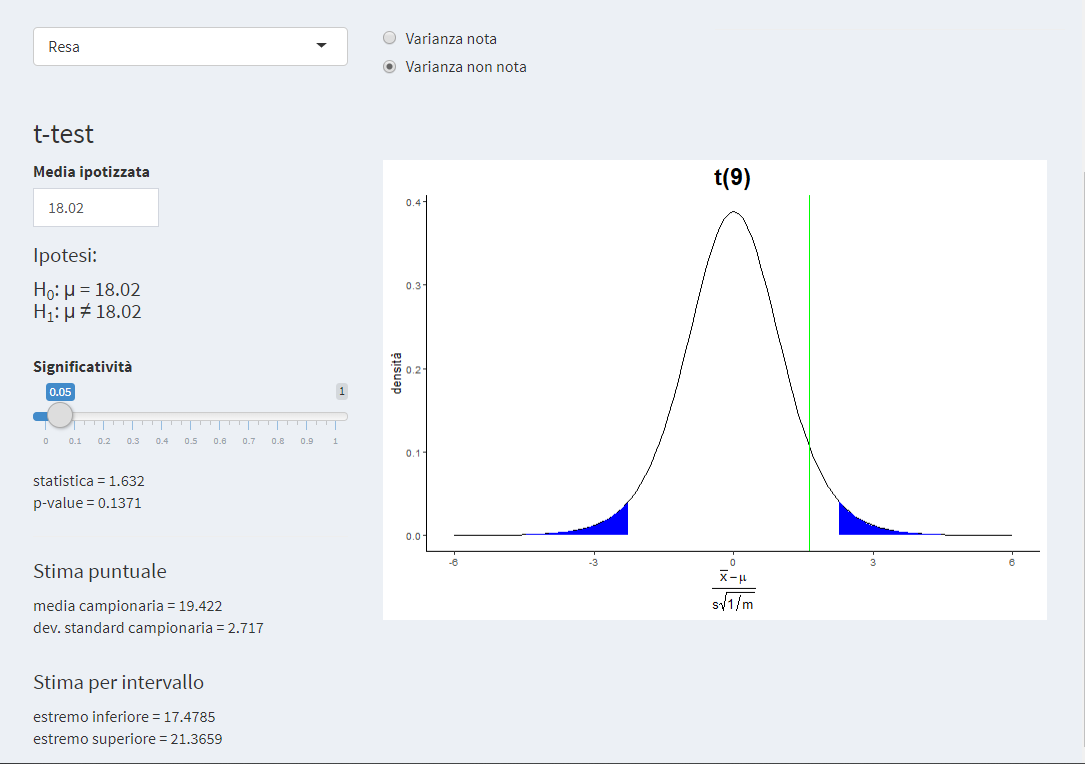
\includegraphics[width=0.5\linewidth]{Immagini/Inferenziale/t_test} \end{center}

\hypertarget{due-popolazioni-gaussiane-campioni-accoppiati}{%
\subsection{Due popolazioni gaussiane: campioni accoppiati}\label{due-popolazioni-gaussiane-campioni-accoppiati}}

Consideriamo il dataset \emph{Diuretico}

\begin{verbatim}
##    Paziente Diuretico.A Diuretico.B
## 1         1         3.5         4.0
## 2         2         4.0         4.2
## 3         3         4.6         4.9
## 4         4         7.1         5.6
## 5         5         3.1         5.1
## 6         6         5.5         5.0
## 7         7         6.8         5.7
## 8         8         5.1         7.1
## 9         9         5.6         6.2
## 10       10         3.8         5.2
## 11       11         4.8         6.3
## 12       12         6.9         6.4
\end{verbatim}

Il dataset consiste nell'elenco dei valori di volume di urina escreta da 12 pazienti volontari a cui sono stati somministrati 2 diuretici differenti qui denominati A e B. La prima colonna della tabella (``Paziente''), riporta il codice identificativo di ogni paziente. Quindi, in questo caso i campioni sono accoppiati in quanto in ogni riga le misure si riferiscono ai volumi di urina raccolti in seguito alla somministrazione del \emph{Diuretico.A} e del \emph{Diuretico.B} allo stesso paziente.

Cade perciò l'ipotesi di indipendenza dei campioni perché, in ciascun paziente, il volume di urina escreto per effetto del diuretico A non è indipendente da quello escreto per effetto del diuretico B: il legame tra i due dati sperimentali è rappresentato dal paziente stesso. Ciascuna coppia di volumi di urina è determinata dalla fisiologia del paziente in esame. Quindi non si può applicare quanto detto finora sui test d'ipotesi e bisogna ridefinire la variabile aleatoria.
Si sceglie quindi di trasformare le \(24\) misure non indipendenti tra loro a coppie, in \(12\) differenze indipendenti tra loro e su questa «nuova» variabile si applica il test più appropriato (\(z\) se sigma nota, \(t\) altrimenti).

Per eseguire il test si procede come segue: una volta caricato il dataset bisogna definire la natura delle variabili (la variabile \emph{Paziente} è qualitativa mentre le altre \(2\) variabili \(Diuretico.A\) e \(Diuretico.B\) sono quantitative) selezionando in Dati/Variabili/Variabili quantitative \emph{Paziente} come variabile qualitativa

\begin{center}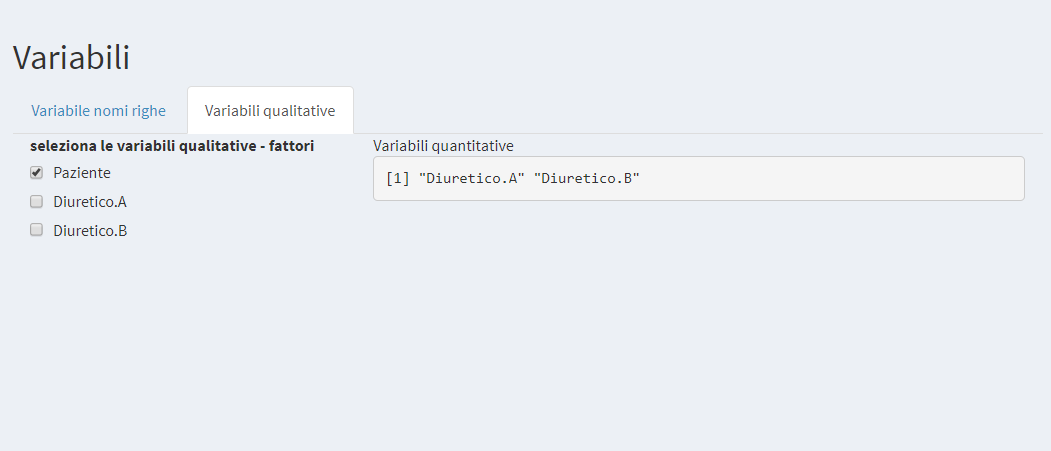
\includegraphics[width=0.5\linewidth]{Immagini/Inferenziale/variabili} \end{center}

Nel menù Statistica inferenziale/Test media si sceglie il caso di due popolazione e si seleziona la pagina Test:dati accoppiati. Non conoscendo a priori la varianza della variabile differenza si clicca su \emph{Varianza non nota}, si indica infine la media della differenza ipotizzata, ad esempio \(\mu_0=0\). Quindi si fissa la significatività \(\alpha\), ad esempio \(\alpha = 0.05\).
Abbiamo evidenza statistica per rifiutare \(H_0\) se la linea verde (che indica il valore \(\frac{\bar{y}-\mu_0}{\sigma\sqrt{1/10}}\) calcolato dal nostro campione) è nella \emph{Regione Critica}, ossia cade nella regione blu. In caso contrario accettiamo \(H_0\) non avendo evidenza statistica per rifiutarla.

Il valore del \emph{p-value} e gli estremi dell'\emph{intervallo di confidenza}, così come il valore della statistica \(\frac{\bar{y}-\mu_0}{\sigma\sqrt{1/10}}\), si ottengono nel menù Statistica inferenziale/Test media: una popolazione

\begin{center}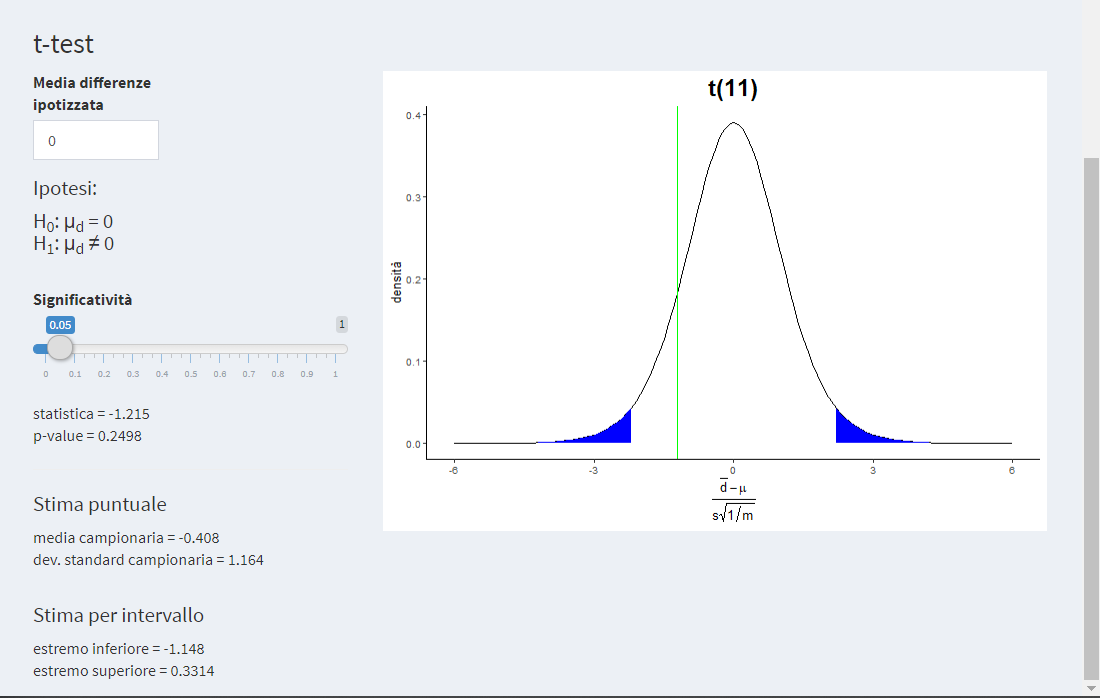
\includegraphics[width=0.5\linewidth]{Immagini/Inferenziale/t_test_accoppiati} \end{center}

\hypertarget{due-popolazioni-gaussiane-campioni-indipendenti}{%
\subsection{Due popolazioni gaussiane: campioni indipendenti}\label{due-popolazioni-gaussiane-campioni-indipendenti}}

Consideriamo il dataset \emph{Resa estrattiva gruppi}

\begin{verbatim}
##        Resa Gruppo
## 1  13.83871      a
## 2  18.76667      b
## 3  17.85000      a
## 4  23.05000      b
## 5  19.26667      a
## 6  20.87097      b
## 7  17.35484      a
## 8  22.37097      b
## 9  21.45000      a
## 10 19.40323      b
\end{verbatim}

che consiste nelle \(10\) misure sperimentali della \emph{Resa estrattiva} considerate nei
paragrafi precedenti a cui è aggiunta una variabile qualitativa (fattore a 2 livelli) \emph{Gruppo} in cui è
indicato il gruppo (pianta \(a\) e pianta \(b\)) a cui appartiene la misura i-esima.

Possiamo rappresentare i dati in 2 colonne (una colonna per pianta) come segue

\begin{verbatim}
##     Resa.a   Resa.b
## 1 13.83871 18.76667
## 2 17.85000 23.05000
## 3 19.26667 20.87097
## 4 17.35484 22.37097
## 5 21.45000 19.40323
\end{verbatim}

Ragionando (colonna per colonna) come fatto nel primo paragrafo, possiamo modellizzare le 5 misure per ogni gruppo come
\[
y_{ia}=\mu_a+\epsilon_{ia} \qquad y_{i5}=\mu_b+\epsilon_{ib}
\]
dove \(\mu_a\) e \(\mu_b\) sono rispettivamente la media ``vera'' della resa estrattiva della pianta \(a\) e la media ``vera'' della resa estrattiva della pianta \(b\) e
\[
\epsilon_{ia}\sim N(0,\sigma_a^2) \qquad  \epsilon_{ib}\sim N(0,\sigma_b^2)
\]
indipendenti.

\hypertarget{varianze-sigma2_a-e-sigma2_b-note}{%
\subsubsection{\texorpdfstring{Varianze \(\sigma^2_a\) e \(\sigma^2_b\) note}{Varianze \textbackslash sigma\^{}2\_a e \textbackslash sigma\^{}2\_b note}}\label{varianze-sigma2_a-e-sigma2_b-note}}

Una stima puntuale di \(\mu_a\) e \(\mu_b\) è data rispettivamente da
\[
\bar y_a = \frac{1}{m_a}\sum_{i=1}^{m_a} y_{aj} \qquad 
\bar y_b = \frac{1}{m_b}\sum_{i=1}^{m_b} y_{bj}
\]

Si può provare che
\[
\frac{(\bar y_a - \bar y_b)-(\mu_a-\mu_b)}{\sqrt{\sigma^2_a/m_a+\sigma^2_b/m_b}} \sim N(0,1)
\]
Si può applicare quanto detto nel primo paragrafo e si usa il \emph{z-test} per valutare la differenza delle medie

\hypertarget{varianze-sigma2_a-e-sigma2_b-non-note}{%
\subsubsection{\texorpdfstring{Varianze \(\sigma^2_a\) e \(\sigma^2_b\) non note}{Varianze \textbackslash sigma\^{}2\_a e \textbackslash sigma\^{}2\_b non note}}\label{varianze-sigma2_a-e-sigma2_b-non-note}}

Se le varianze non sono note, si deve stimare anche la varianza e in questo si può usare la media ponderata delle varianze dei due campioni che è uno stimatore migliore delle singole varianze di ciascun campione.
Introduciamo la \emph{varianza combinata}
\[
s_c^2 = \frac{(m_a+1)s_a^2+(m_b+1)s_b^2}{m_a+m_b-2}.
\]

Si può dimostrare che se \(\sigma^2_a=\sigma^2_b\)

\[
\frac{(\bar y_a - \bar y_b)-(\mu_a-\mu_b)}{s_c\sqrt{1/m_a+1/m_b}} \sim t(m_a+m_b-2)
\]

mentre nel caso in cui non possiamo supporre che le varianze siano uguali i gradi di libertà \(\nu\) della distribuzione \(t\) possono essere approssimati dalla \emph{formula di Welch}
\[
\nu \approx \frac{\frac{s^2_a}{m_a}+\frac{s^2_b}{m_b}}{\frac{s^2_a}{m_a^2(m_a-1)}+\frac{s^2_b}{m_b^2(m_b-1)}}
\]
e quindi

\[
\frac{(\bar y_a - \bar y_b)-(\mu_a-\mu_b)}{s_c\sqrt{1/m_a+1/m_b}} \sim t(\nu)
\]

I gradi di libertà stimati dalla \emph{formula di Welch} sono minori dei gradi di libertà nel caso in cui le varianze siano uguali. Il test risulta quindi ``meno potente nel distinguere le medie''.\\
Vediamo quanto detto con il nostro esempio.

Per eseguire il test si procede come segue: una volta caricato il dataset bisogna definire la natura delle variabili (la variabile \emph{Gruppo} è qualitativa mentre la variabile \(Resa\) è quantitativa) selezionando in Dati/Variabili/Variabili quantitaive \emph{Gruppo} come variabile qualitativa.

Nel menù Statistica inferenziale/Test media si sceglie il caso di due popolazioni e si seleziona la pagina Test:dati indipendenti. Non conoscendo a priori le varianze si clicca su \emph{Varianza non nota}, e quindi scegliere l'opzione Varianze uguali/Varianze non uguali a seconda del caso (nel paragrafo successivo descriviamo un test per la verifica dell'uguaglianza delle variabili).
Si fissa la significatività \(\alpha\), ad esempio \(\alpha = 0.05\) e si prosegue come già visto (figura a sinistra caso varianze uguali, figura a destra varianze non uguali)

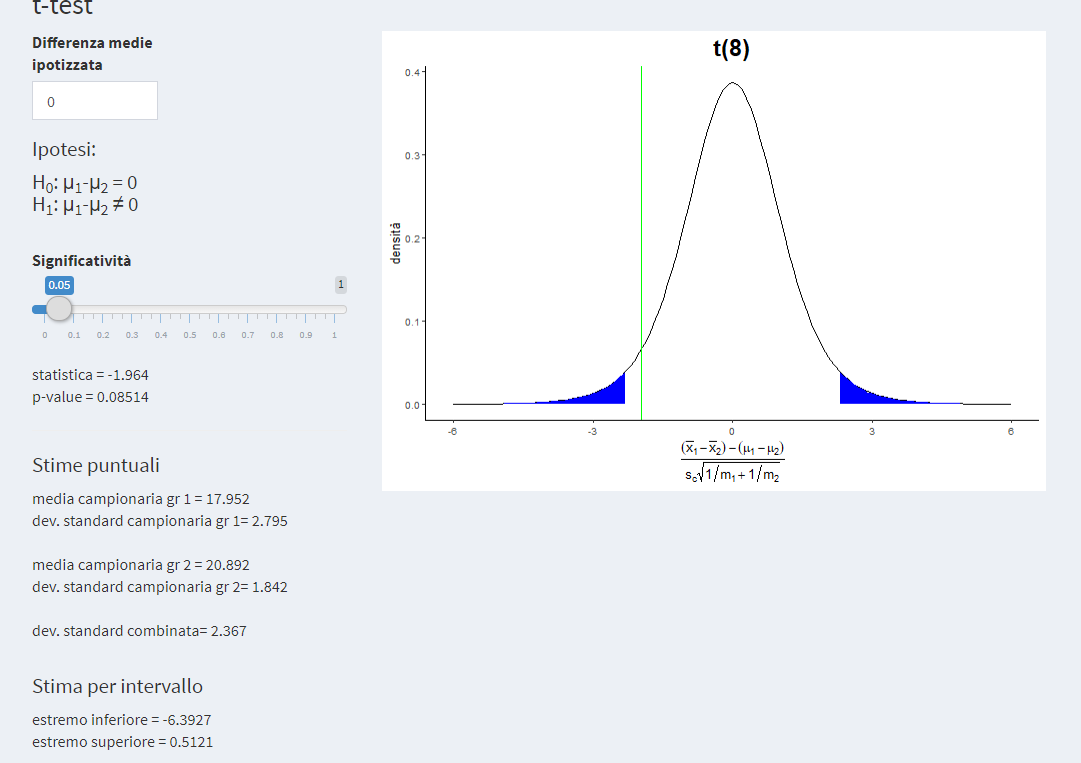
\includegraphics[width=0.5\linewidth]{Immagini/Inferenziale/t_test_indip_1}
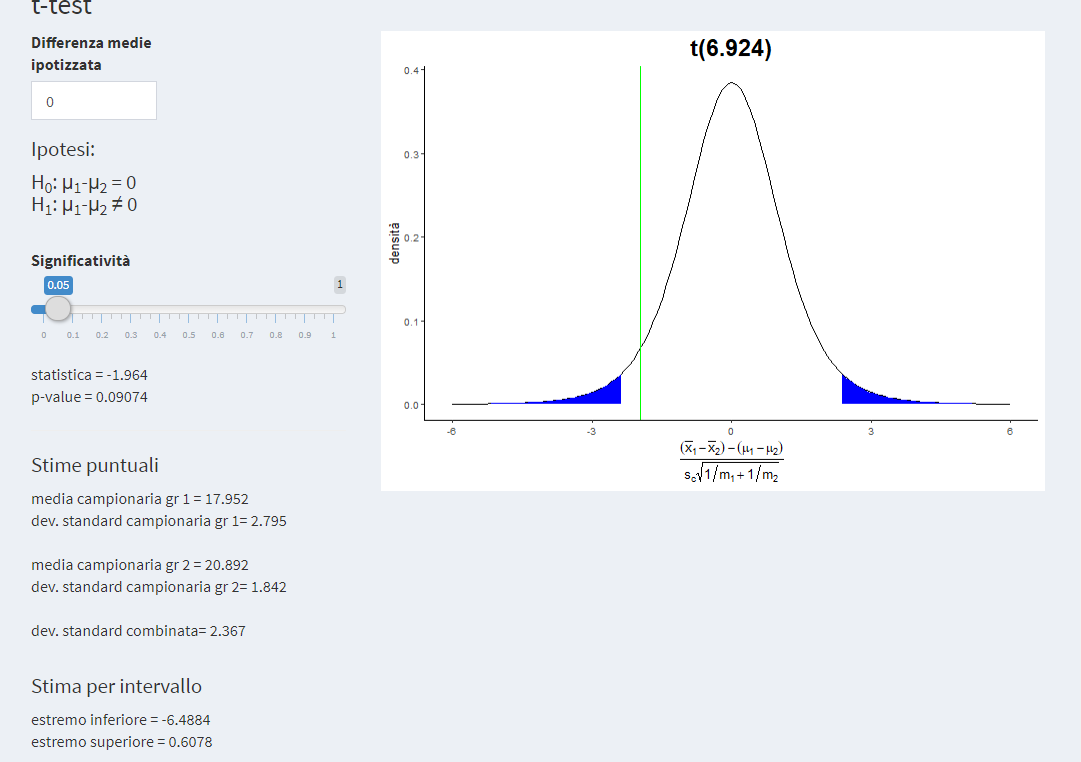
\includegraphics[width=0.5\linewidth]{Immagini/Inferenziale/t_test_indip_2}

I gradi di libertà stimati dalla \emph{formula di Welch} sono \(\nu = 6 . 924\) (figura a destra) minori di \(8\) (gradi di libertà
nel caso in cui le varianze siano uguali). Come già osservato il test è quindi ``meno potente nel distinguere le medie''.
Questo lo si nota dal valore del \emph{p-value} che risulta maggiore e dall'intervallo di confidenza che risulta più ampio.

\hypertarget{f-test}{%
\paragraph{F-test}\label{f-test}}

Per quanto appena visto abbiamo bisogno di verificare l'ipotesi di uguaglianza delle varianze dei due campioni.

E' nota la distribuzione del rapporto tra la stima delle varianze e le varianze di popolazione:
\[
\frac{s^2_a/\sigma^2_a}{s^2_b/\sigma^2_b} \sim F(m_a-1,m_b-1)
\]
Si tratta della distribuzione F di Fisher (in figura per alcune combinazioni di gradi di libertà)

\begin{center}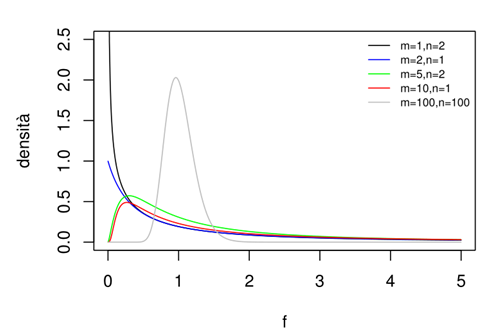
\includegraphics[width=0.5\linewidth]{Immagini/Inferenziale/distr_f} \end{center}

Ragionando in maniera analoga a quanto fatto nel capitolo per i test \(t\) e \(z\) possiamo eseguire il cosiddetto \(F-test\) delle varianze
\[
H_0: \sigma^2_a=\sigma^2_b  \quad \rm{vs} \quad H_1: \sigma^2_a \neq \sigma^2_b 
\]
L'intervallo di confidenza è definito

\[
\frac{s^2_a}{s^2_b}\frac{1}{f_{\alpha/2}} \leq \frac{\sigma^2_a}{\sigma^2_b} \leq 
\frac{s^2_a}{s^2_b}\frac{1}{f_{1-\alpha/2}}
\]
dove \(f_{\alpha/2}\) indica il quantile di ordine \(1-\alpha/2\) della distribuzione \(F(m_a-1,m_b-1)\),
i.e.~\(\mathbb{P}[f \geq f_{\alpha/2}]=\alpha/2\), \(f\sim F(m_a-1,m_b-1)\).

Per meglio comprendere, vediamo come eseguire il test.\\
Nel menù Statistica inferenziale/Test test varianza:due popolazioni si fissa la significatività \(\alpha\), ad esempio \(\alpha = 0.05\).
Abbiamo evidenza statistica per rifiutare \(H_0\) se la linea verde (che indica il valore \(s_a^2/s_b^2\) calcolato dal nostro campione) è nella \emph{Regione Critica}, ossia cade nella regione blu. In caso contrario accettiamo \(H_0\) non avendo evidenza statistica per rifiutarla.

\begin{center}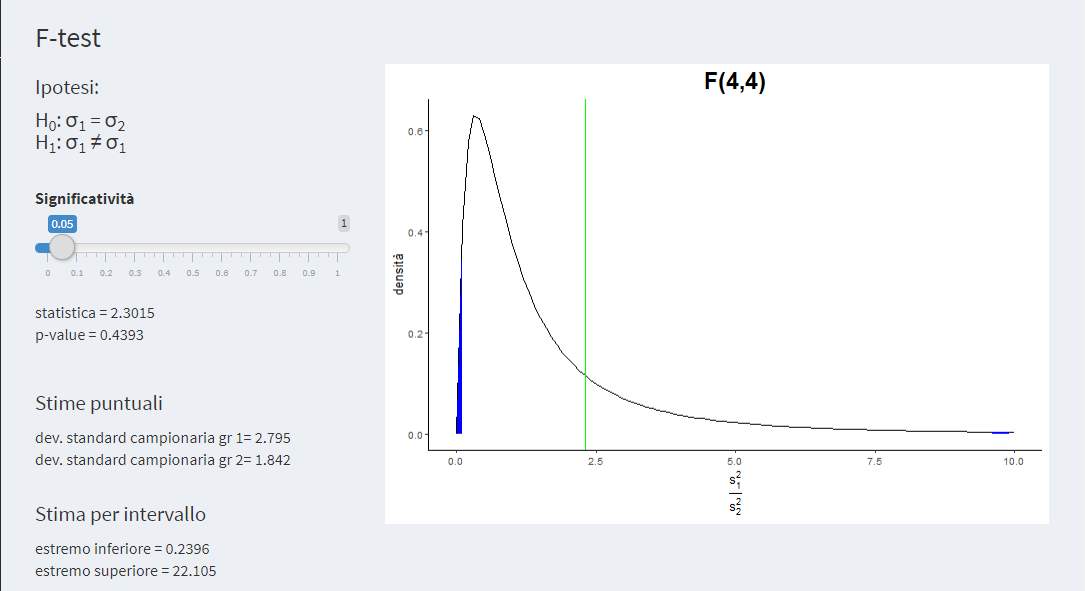
\includegraphics[width=0.5\linewidth]{Immagini/Inferenziale/f_test} \end{center}

Si ottengono il valore del \emph{p-value} e gli estremi dell'\emph{intervallo di confidenza}.

Si noti che in questo caso stiamo verificando l'ipotesi nulla che postula che il rapporto tra le varianze è uguale a 1. Ragionando per intervallo di confidenza abbiamo evidenza statistica per rifiutare \(H_0\) se tale intervallo non contiene \(1\), in caso contrario non abbiamo evidenza per rifiutare \(H_0\).

\hypertarget{regressione-lineare-semplice}{%
\chapter{Regressione lineare semplice}\label{regressione-lineare-semplice}}

Ricordiamo brevemente l'equazione di una retta su un piano di coordinate \((x,y)\):
\[
y=\beta_0+\beta_1x
\]
il cui grafico è dato da

\begin{center}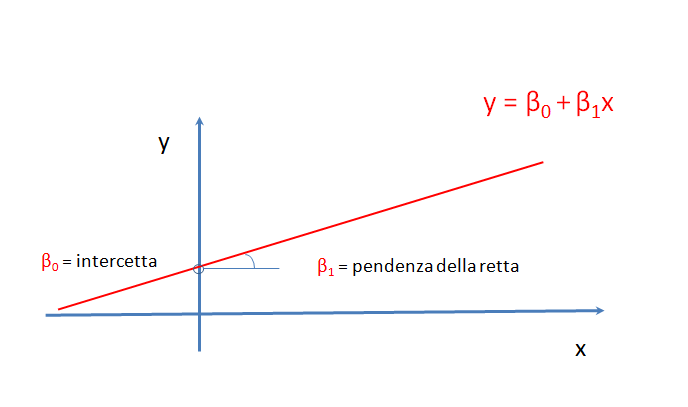
\includegraphics[width=0.5\linewidth]{Immagini/Regressione/01_graf_retta} \end{center}

dove \(\beta_0\) è l'intercetta, ossia il valore della \(y\) per \(x=0\), e \(\beta_1\) è la pendenza della retta e indica di quanto cresce (o decresce) la \(y\) all'aumentare di un'unità nella \(x\).

Supponiamo ora di dover costruire la retta di taratura (i.e.~determinare i parametri \(\beta_0\) e \(\beta_1\)) di uno strumento per la determinazione delle proteine totali in colture cellulari. L'esperimento consiste nel leggere l'assorbanza misurata \(y\) da uno spettofotometro per concentrazioni note \(x\). I dati sperimentali sono indicati nella seguente tabella

\begin{verbatim}
##   Concentrazione Assorbanza
## 1            100      2.298
## 2             80      2.018
## 3             50      1.618
## 4             40      1.383
## 5             20      0.882
\end{verbatim}

I 5 risultati sperimentali della tabella sono un campione della popolazione di tutti gli esperimenti teoricamente possibili, e a partire da questo campione vogliamo stimare i parametri \(\beta_0\) e \(\beta_1\).

I 5 risultati sperimentali li rappresentiamo nel piano \((concentrazione,assorbanza)\)

\begin{center}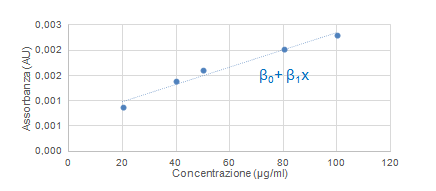
\includegraphics[width=0.5\linewidth]{Immagini/Regressione/02_graf_dati} \end{center}

La retta tratteggiata è la retta di taratura i cui parametri vogliamo stimare a partire dal campione delle 5 misure sperimentali date.

Ragionando in maniera simile a quanto fatto nel capitolo \emph{Statistica inferenziale} per la media, possiamo supporre che la misura sperimentale \(y\) per un livello di concentrazione \(x\) fissato differisca dal risultato terorico ``vero'' \(\beta_0+\beta_1x\) per un errore sperimentale \(\epsilon\) puramente casuale
\[
y=\beta_0+\beta_1x + \epsilon
\]
e che l'errore sperimentale \(\epsilon\) sia distribuito come una normale di media 0 e varianza \(\sigma^2\)
\[
\epsilon \sim N(0,\sigma^2)
\]
Si noti che la varianza \(\sigma^2\) è ipotizzata sempre uguale per tutte le misure (ipotesi di omoschedasticità).\\
N.B. Ciò significa, sul piano pratico, che le 5 misure dei valori di y abbiano uguale precisione (in senso strettamente analitico, la precisione si rappresenta con il coefficiente di variazione che è la deviazione standard relativa\%).

Altra importante ipotesi è che le misure siano indipendenti le une dalle altre, ossia che il risultato di ogni misura (ad es. \(y_1\))
non è influenzato in alcun modo da una misura precedente o successiva (ad es. \(y_2\)).

\hypertarget{stima-dei-parametri-beta_0-e-beta_1}{%
\section{\texorpdfstring{Stima dei parametri \(\beta_0\) e \(\beta_1\)}{Stima dei parametri \textbackslash beta\_0 e \textbackslash beta\_1}}\label{stima-dei-parametri-beta_0-e-beta_1}}

Data una retta qualsiasi del piano \(y=b_0+b_1x\), indichiamo con \(e_i\) la differenza tra i 5 valori misurati \(y_i\) e i 5 valori \(b_0+b_1x_i\)
\[
e_i=y_i-(b_0+b_1x_i)
\]

indicate con le frecce rosse in figura

\begin{center}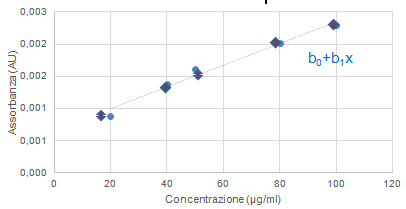
\includegraphics[width=0.5\linewidth]{Immagini/Regressione/04_min_sq} \end{center}

Si può dimostrare, (v. \textbf{metodo dei minimi quadrati} nel Glossario), che esiste una unica retta \(y=\hat{\beta_0}+\hat{\beta_1}x\) che minimizza la somma dei quadrati \(\sum_{i=1}^m e_i^2\) (\(m=5\) nel nostro esempio) e che i valori \(\hat{\beta_0}\) e \(\hat{\beta_1}\) sono dati da
\begin{eqnarray*}
\hat{\beta_1}&=&\frac{\sum_{i=1}^m (x_i-\bar{x})(y_i-\bar{y})}{\sum_{i=1}^m(x_i-\bar{x})^2} \\
\hat{\beta_0}&=&\bar{y}-\hat{\beta}_1\bar{x}.
\end{eqnarray*}

I valori \(\hat{\beta_0}\) e \(\hat{\beta_1}\) dipendono dal campione di 5 misure, un nuovo campione porta a valori diversi. Sono variabili aleatorie.

Si verifica facilmente che \(\hat{\beta_0}\) e \(\hat{\beta_1}\) sono una stima puntuale dei parametri \(\beta_0\) e \(\beta_1\), cioè ripetendo un gran numero di esperimenti ``in media'' \(\hat{\beta_0}\) e \(\hat{\beta_1}\) tendono a coincidere con il valore «vero» \(\beta_0\) e \(\beta_1\).\\
N.B. Questo concetto, si rappresenta formalmente con la media, o speranza matematica di una variabile casuale (ad es. \(\beta_0\)), e si indica con

\[
\mathbb{E}(\hat{\beta_0})=\beta_0 \quad \rm{e} \quad \mathbb{E}(\hat{\beta_1})=\beta_1
\]
in cui la notazione
\[
\mathbb{E}()
\]
deriva da \emph{expected} o \emph{expectation} in inglese o dal francese \emph{espérance}, e formalizza il concetto di valore medio di un fenomeno aleatorio.

E' nota anche la precisione di questi stimatori, infatti si può dimostrare che

\begin{eqnarray*}
\rm{Var}(\hat{\beta_0})&=&[\frac{1}{m}+\frac{\bar{x}^2}{\sum_{i=1}^m(x_i-\bar{x})^2}]\sigma^2\\
\rm{Var}(\hat{\beta_1})&=&\frac{\sigma^2}{\sum_{i=1}^m(x_i-\bar{x})^2} .
\end{eqnarray*}

Si noti che le varianze degli stimatori non dipendono dai risultati sperimentali \(y_i\), sono anche chiamate «errore standard» degli stimatori (Excel). Sono determinate a priori -- vale a dire che dipendono solo dal piano sperimentale.
Inoltre si noti che sono inversamente proporzionali a \(\sum_{i=1}^m(x_i-\bar{x})^2\), cioè alla misura della ``dispersione'' delle \(x\).

Le stime puntuali, una volta caricato il dataset, si ottengono nel menù Regressione lineare/semplice

\begin{center}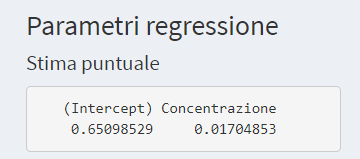
\includegraphics[width=0.5\linewidth]{Immagini/Regressione/05_stima_pt} \end{center}

\hypertarget{significativituxe0-dei-coefficienti}{%
\section{Significatività dei coefficienti}\label{significativituxe0-dei-coefficienti}}

Per fare inferenza a partire dalle 5 misure campionarie, abbiamo bisogno di conoscere la distribuzione di probabilità degli stimatori \(\hat{\beta_0}\) e \(\hat{\beta_1}\). Abbiamo innanzitutto bisogno di stimare la varianza \(\sigma^2\). Una stima puntuale è data da:
\[
s^2=\frac{\sum_{i=1}^m[y_i-(\hat{\beta_0} + \hat{\beta_1}x_1)]^2}{m-2}
\]
Si può dimostrare che

\begin{eqnarray*}
\frac{\hat{\beta_0}-\beta_0}{s\sqrt{h}}&\sim&t(m-2)\\
\frac{\hat{\beta_1}-\beta_1}{s\sqrt{1/S^2_{x}}}&\sim&t(m-2),
\end{eqnarray*}
dove \(h=\frac{1}{m}+\frac{\bar{x}^2}{S^2_{x}}\) e \(S^2_{x}=\sum_{i=1}^m(x_i-\bar{x})^2\).

Ragionando come fatto nel capitolo precedente per la media possiamo verificare la significatività dei coefficienti al \(1-\alpha\%\) (\(\alpha=0.05\) in generale):

\begin{itemize}
\tightlist
\item
  test ipotesi (\emph{t-test})
\end{itemize}

\begin{eqnarray*}
H_0: \beta_0=0 \quad & \rm{vs} & \quad H_0: \beta_0\neq0 \\
H_0: \beta_1=0 \quad & \rm{vs} & \quad H_1: \beta_0\neq0
\end{eqnarray*}

\begin{itemize}
\tightlist
\item
  intervallo di confidenza
  \begin{eqnarray*}
  % \nonumber to remove numbering (before each equation)
  \hat\beta_0 & \pm & t(\alpha/2,m-2)s\sqrt{h} \\
  \hat\beta_1 & \pm & t(\alpha/2,m-2)s\sqrt{1/S^2_{x}}
  \end{eqnarray*}
\end{itemize}

Sempre dal menù Regressione lineare/semplice otteniamo gli estremi degli intervalli di confidenza al 95\%

\begin{center}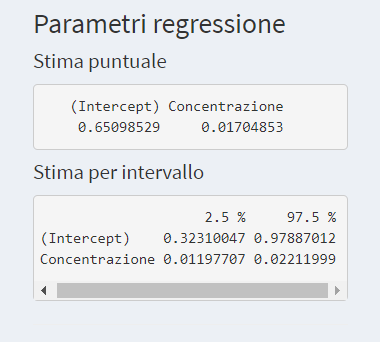
\includegraphics[width=0.5\linewidth]{Immagini/Regressione/06_stima_interv} \end{center}

Se l'intervallo di confidenza contiene lo 0 non possiamo affermare che il parametro è significativamente diverso da 0, nel caso contrario possiamo affermare che il parametro è significativo. Nell'esempio considerato, sia l'intercetta che la pendenza sono significativamente diversi da 0.

Nella stessa pagina abbiamo anche il seguente output

\begin{center}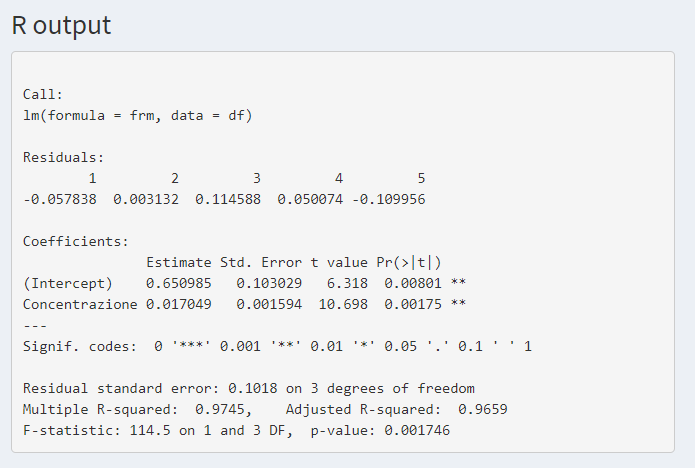
\includegraphics[width=0.5\linewidth]{Immagini/Regressione/07_R_output} \end{center}

in cui sono riportati oltre al valore dei residui \(y_i-(\hat{\beta_0}+\hat{\beta_1}x_i)\), la stima dei parametri \(\hat{\beta_0}\) e \(\hat{\beta_1}\), il loro errore standard \(s\sqrt{h}\) e \(s\sqrt{1/S^2_{x}}\) rispettivamente, le statistiche \(t\)
\[
\frac{\hat{\beta_0}}{s\sqrt{h}}, \qquad \qquad \frac{\hat{\beta_1}}{s\sqrt{1/S^2_{x}}}
\]

e il \emph{p-value} dei \emph{t-test} (vedi il capitolo precedente per la definizione).

Nell'output nella figura precedente viene riportata la stima di \(\sigma\) \emph{Residual standard error} con i relativi gradi di libertà. E' riportato anche il valore di \(R^2\), un indicatore che misura quanto la variazione di \(y\) è descritta dalla variazione di \(x\) attraverso la relazione funzionale studiata, (\(R^2\) è un indice di \emph{fitting}, adattamento).

\hypertarget{previsione-del-modello}{%
\section{Previsione del modello}\label{previsione-del-modello}}

In questo paragrafo ci occupiamo della stima dell'assorbanza ``vera'' \(y_0=\beta_0+\beta_1x_0\) per un valore di concentrazione \(x_0\).

\begin{center}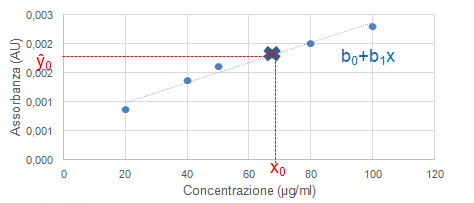
\includegraphics[width=0.5\linewidth]{Immagini/Regressione/08_prev} \end{center}

La stima puntuale della previsione è data da:
\[
\hat{y_0}=\hat{\beta_0}+\hat{\beta_1}x_0
\]
Il valore di tale stima dipende ovviamente dal campione di 5 misure; un nuovo campione porta ad un valore diverso della stima ma questa, ``in media'', ripetendo un gran numero di esperimenti, tende al valore ``vero'' \(y_0=\beta_0+\beta_1x_0\).

\[
\mathbb{E}(\hat{y_0})=y_0
\]

Si osservi che il ``valore vero'' non è il valore di una misura in \(x_0\) che è affetta da errore, ma la ``media'' di un gran numero di misure in \(x_0\).

E' nota la precisione dello stimatore \(\hat{y_0}\):
\[
\rm{Var}(\hat{y_0})=[\frac{1}{m}+\frac{(x_0-\bar{x})^2}{S^2_{x}}]\sigma^2
\]
Il valore \(h_0=\frac{1}{m}+\frac{(x_0-\bar{x})^2}{S^2_{x}}\) è chiamato valore leva (\emph{leverage}) per il punto \(x_0\) ed è un indicatore della qualità dello stimatore \(\hat{y_0}\).
L'unico parametro controllabile da cui dipende la precisione della previsione è \(S^2_{x}\). Più grande è tale valore migliori sono le stime.
Poiché \(S^2_{x}\) misura lo ``spread'' delle \(x\), è una buona idea quando si progetta un esperimento allargare il range delle \(x\) il più possibile. Inoltre aumentando i valori delle \(x\) verso gli estremi del range, si aumenta ulteriormente \(S^2_{x}\).

In figura è indicato con la linea rossa il leverage per ogni valore di concentrazione nel range del nostro esempio, mentre è indicato con una linea verde il leverage con un ``disegno sperimentale'' leggermente modificato aumentando lo ``spread'' delle \(x\) (i 5 campioni sono per le seguenti concentrazioni: 100, 100, 50, 20, 20)

\begin{center}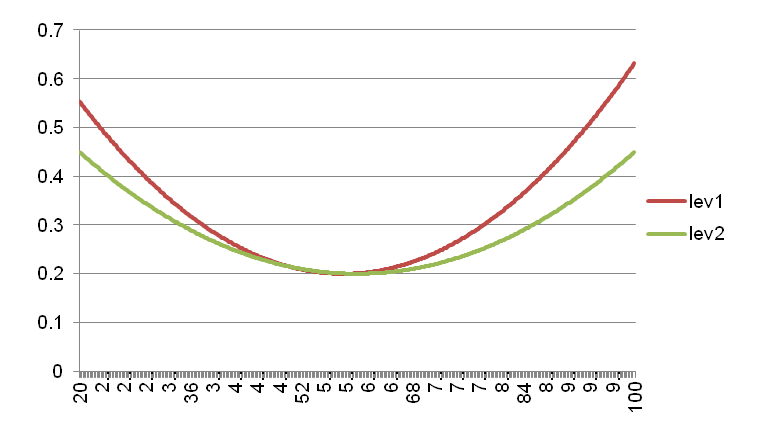
\includegraphics[width=0.5\linewidth]{Immagini/Regressione/11_lev} \end{center}

Si noti inoltre che a differenza dei modelli per la media visti nel capitolo precedente in cui il valore ``leva'' dipendeva dal numero di osservazioni nel punto, per la regressione lineare dipende anche dalla ``posizione'' del punto rispetto alla media.

Altra importante osservazione da fare è che il leverage non dipende dai risultati sperimentali ma dipende soltanto da come sono stati progettati gli esperimenti.

Si può dimostrare che
\[
\frac{\hat{y_0}-y_0}{s\sqrt{\frac{1}{m}+\frac{(x_0-\bar{x})^2}{S^2_{x}}}}\sim t(m-2).
\]

Ragionando come in precedenza possiamo quindi definire il seguente \emph{intervallo di confidenza} (stima per intervallo della previsione)
\[
\hat{y_0}\pm t(\alpha/2,m-2)s\sqrt{\frac{1}{m}+\frac{(x_0-\bar{x})^2}{S_{xx}}}
\]

Nella seguente figura (ottenuta in Regressione lineare/semplice) è rappresentato l'intervallo di confidenza (zona grigia) per i valori di concentrazione nel range del nostro esempio.

\begin{center}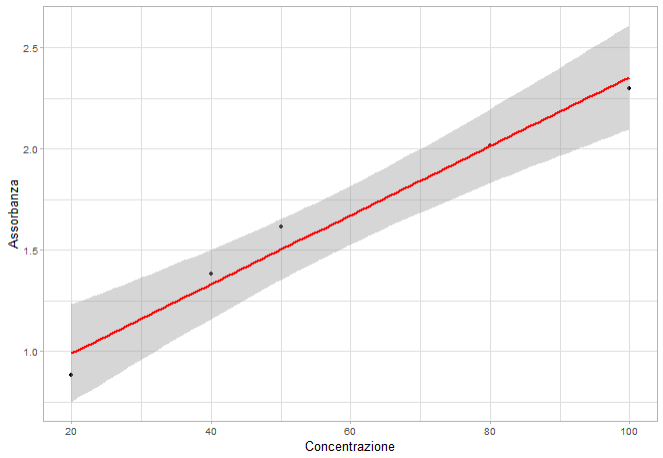
\includegraphics[width=0.5\linewidth]{Immagini/Regressione/09_int_conf_prev} \end{center}

Si noti che, per quanto osservato in precedenza sul leverage, l'intervallo è ``più stretto'' nella parte centrale del range e quindi la ``qualità'' della previsione è migliore in quella regione del range.

In Regressione lineare/semplice, fissato il valore \(x_0\) della concentrazione viene fornito l'intervallo di confidenza (al 95\%) della previsone dell'assorbanza

\begin{center}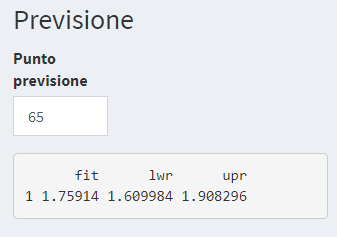
\includegraphics[width=0.5\linewidth]{Immagini/Regressione/10_int_conf_prev_numerico} \end{center}

\hypertarget{verifica-delle-ipotesi-1}{%
\section{Verifica delle ipotesi}\label{verifica-delle-ipotesi-1}}

Affinché quanto detto sia valido, in particolare per quanto riguarda l'inferenza sui parametri e sulla stima, dobbiamo verificare che siano soddisfatte le ipotesi formulate all'inizio di questo capitolo: tali ipotesi erano che i residui sulle y fossero distribuiti secondo la normale (di media 0), che avessero varianze non troppo differenti tra loro (omoschedasticità) e che fossero indipendenti tra loro.

Nel menù Regressione lineare/semplice alla pagina \emph{Verifica ipotesi} sono proposti i seguenti test e grafici:

\begin{itemize}
\tightlist
\item
  \textbf{Media nulla}\\
  sono proposti un \emph{t-test} in cui l'ipotesi nulla è che la media dei residui sia 0 (la media non è significativamente diversa da 0 per valori del \emph{p-value} più grandi di \(\alpha\) = 0.05) e un grafico dei residui vs i valori predetti (in cui i residui devono essere distribuiti casualmente intorno alla retta orizzontale tratteggiata per convalidare l'ipotesi di indipendenza). Da questo grafico si possono osservare eventuali deviazioni dalla linearità del modello. Se la nuvola dei punti plottati assume qualche particolare forma, ad esempio di parabola, si ha la prova della esistenza di deviazione dalla linearità.
\end{itemize}

\begin{center}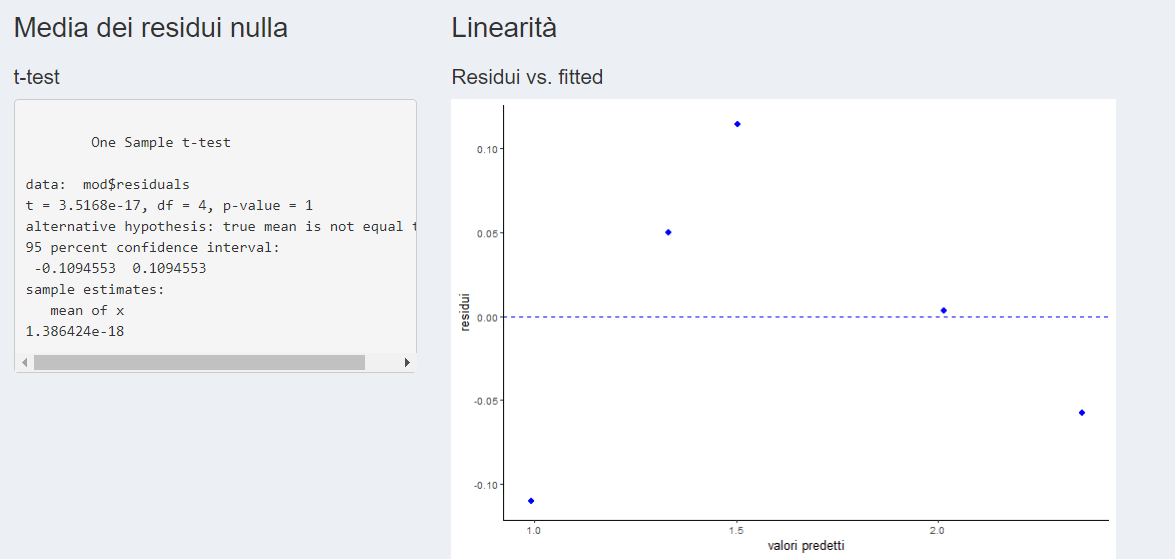
\includegraphics[width=0.5\linewidth]{Immagini/Regressione/12_ipotesi1} \end{center}

\begin{itemize}
\tightlist
\item
  \textbf{Normalità}\\
  Viene proposto il \emph{test di Shapiro Wilk}, uno dei test più potenti per la normalità soprattutto per piccoli campioni: l'ipotesi nulla è che la distribuzione sia normale. La normalità è verificata per valori grandi del \emph{p-value} (\(> \alpha = 0.05\)). Si calcola la statistica \emph{W} (\(0<W<1\)), data dal rapporto di due stimatori alternativi di \(\sigma^2\). Se la distribuzione è normale la statistica W risulta prossima a 1. Viene anche proposto il \emph{QQ-Plot} in cui sono rappresentati i quantili del campione vs i quantili teorici di una distribuzione normale. Se la distribuzione dei dati del campione è normale i quantili campionari sono avviluppati intorno alla retta tratteggiata.
\end{itemize}

\begin{center}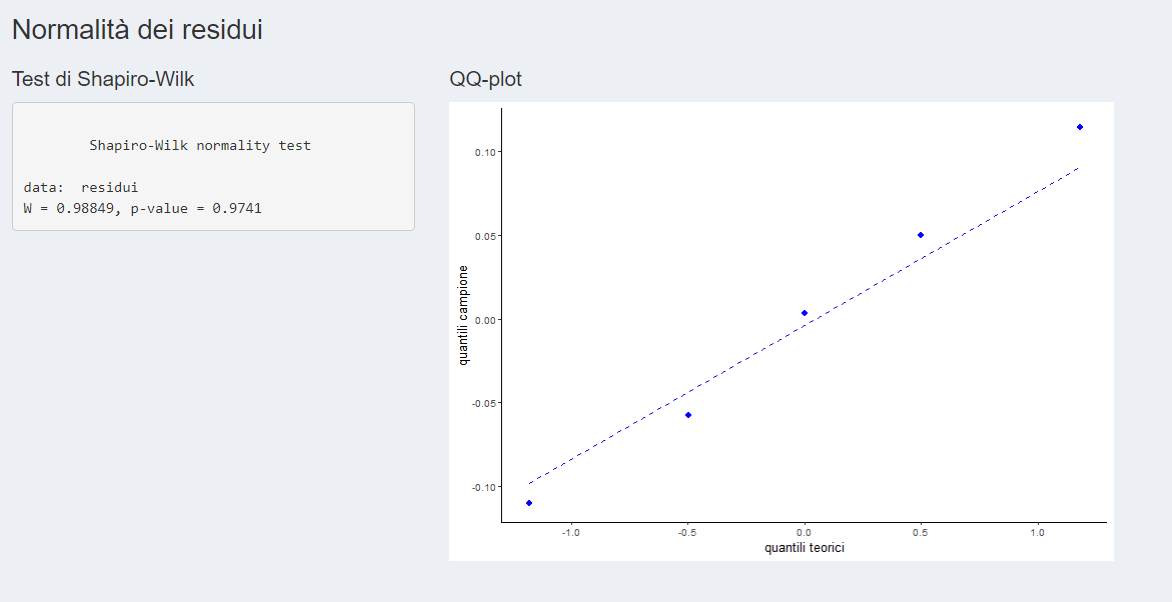
\includegraphics[width=0.5\linewidth]{Immagini/Regressione/13_ipotesi2} \end{center}

\begin{itemize}
\tightlist
\item
  \textbf{Omoschedasticità}\\
  Viene proposto il \emph{test di Breusch Pagan} la cui ipotesi nulla è l'omoschedasticità dei residui. La omoschedasticità è verificata per valori grandi del \emph{p-value} (\(>\alpha = 0.05\))). E' anche proposto un grafico della radice dei residui vs i valori predetti.
  In caso di eteroschedasticità nel grafico risulta evidente una tendenza di dispersione, ad esempio crescente, con la nuvola dei punti che assume una forma a cono, cosa che non accade in caso di omoschedasticità degli errori.
\end{itemize}

\begin{center}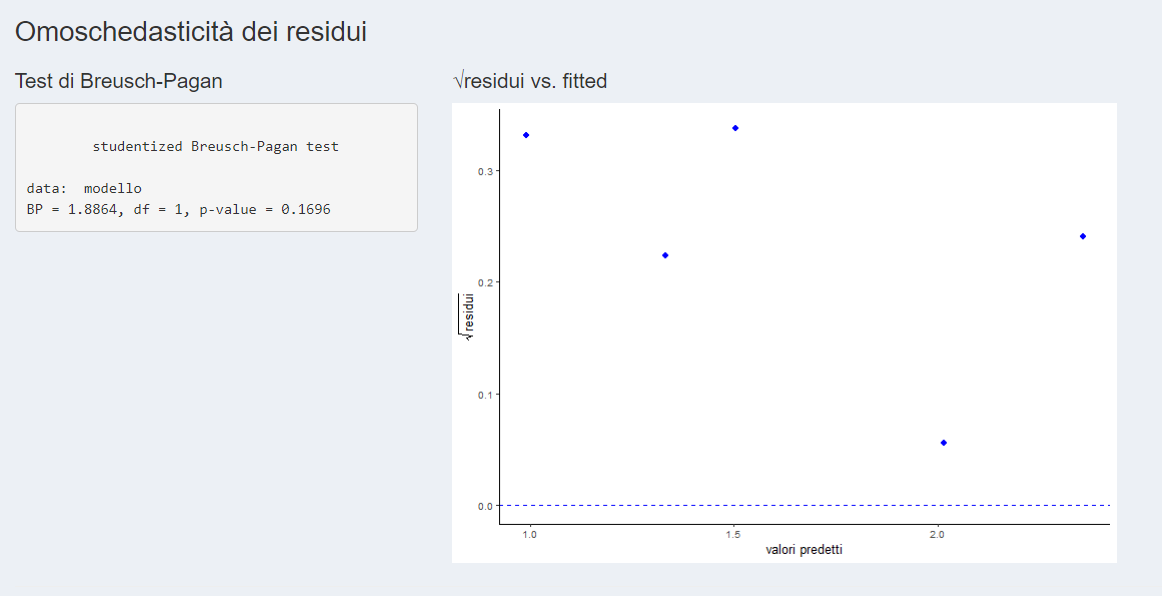
\includegraphics[width=0.5\linewidth]{Immagini/Regressione/14_ipotesi3} \end{center}

\begin{itemize}
\tightlist
\item
  \textbf{Correlazione seriale}\\
  Viene proposto il \emph{test di Durbin-Watson} per valutare la presenza di autocorrelazione tra i dati. L'ipotesi nulla è la assenza di autocorrelazione dei residui. La assenza di autocorrelazione è verificata per valori grandi del \emph{p-value} (\(> \alpha = 0.05\)). Il grafico che è stampato insieme alla statistica del test mostra il residuo n-esimo vs il residuo (n-1)-esimo e serve a mettere in evidenza la eventuale correlazione seriale degli errori.
\end{itemize}

\begin{center}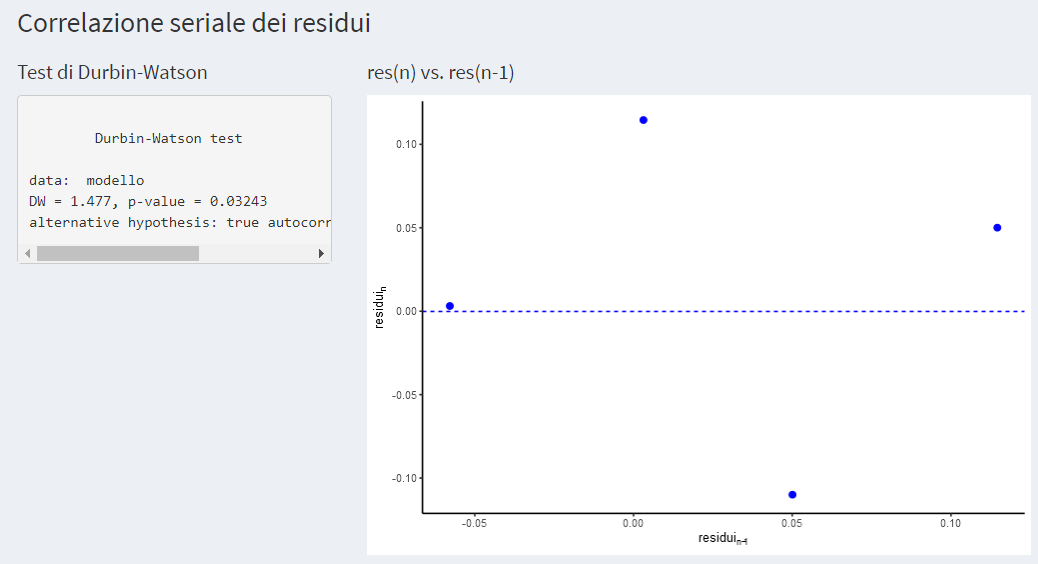
\includegraphics[width=0.5\linewidth]{Immagini/Regressione/15_ipotesi4} \end{center}

\hypertarget{analisi-della-varianza}{%
\chapter{Analisi della Varianza}\label{analisi-della-varianza}}

\hypertarget{analisi-della-varianza-a-un-fattore}{%
\section{Analisi della varianza a un fattore}\label{analisi-della-varianza-a-un-fattore}}

Consideriamo il dataset \emph{Collirio}

\begin{verbatim}
##   Nessuna    A.R    A5s   A10s
## 1  0.0285 0.0377 0.0677 0.0920
## 2  0.0304 0.0346 0.0604 0.0934
## 3  0.0295 0.0369 0.0673 0.0948
## 4  0.0318 0.0439 0.0674 0.1011
## 5  0.0303 0.0485 0.1073 0.0833
## 6  0.0315 0.0488 0.1138 0.0909
## 7  0.0322 0.0648 0.1210 0.0987
## 8  0.0315 0.0743 0.1330 0.1080
\end{verbatim}

che consiste in 32 misure sperimentali (\emph{Pesata}) della massa di una goccia di un collirio preparato prima dell'uso in 4
modi diversi, indicati nelle colonne della tabella; questa ultima variabile (\emph{Preparazione}) è un \emph{fattore} qualitativo studiato a 4 livelli: Nessuna, A.R., A5s, A10s.

Possiamo modellizzare le 8 misure per ogni tipo di \emph{Preparazione} come
\[
y_{i1}=\mu+\alpha_1+\epsilon_{i1} \qquad y_{i2}=\mu+\alpha_2+\epsilon_{i2} \qquad y_{i3}=\mu+\alpha_3+\epsilon_{i3} \qquad y_{i4}=\mu+\alpha_4+\epsilon_{i4}
\]
dove \(\mu+\alpha_i\) è la media ``vera'' della \emph{Pesata} con \(\mu\) parametro comune a tutti gli effetti, detta media complessiva, e \(\alpha_1, \alpha_2, \alpha_3\) e \(\alpha_4\) sono i contributi nella media ``vera'' dovuti all'effetto della \emph{Preparazione}: Nessuna, A.R., A5s, A10s. Inoltre gli errori casuali
\[
\epsilon_{i1}\sim N(0,\sigma^2) \qquad \epsilon_{i2}\sim N(0,\sigma^2) \qquad \epsilon_{i3}\sim N(0,\sigma^2) \qquad \epsilon_{i4}\sim N(0,\sigma^2)
\]
sono a due a due non correlati tra loro. Si noti che è richiesto che abbiano tutti la stessa varianza \(\sigma^2\) (ipotesi di omoschedasticità).

Cominciamo con l'importare in Dati/Esempi Master il dataset \emph{Collirio}. In ``Variabili'' nella pagina ``Variabili qualitative'' bisogna selezionare la variabile \emph{Preparazione} (fattore qualitativo a 4 livelli)

\begin{center}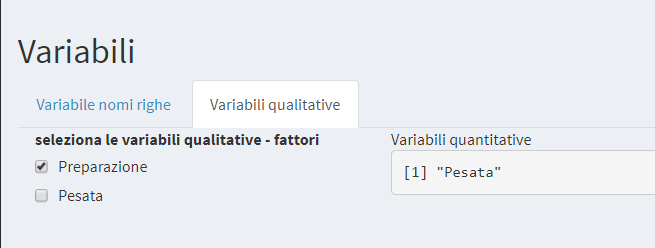
\includegraphics[width=0.5\linewidth]{Immagini/Anova/01_var_quali} \end{center}

Esaminiamo l'effetto del fattore \emph{Preparazione} sulla \emph{Pesata}. Per avere una prima idea grafica possiamo, in ``Statistica descrittiva/Box plot'', ottenere i box plot delle quattro colonne di dati.

\begin{center}\includegraphics[width=0.5\linewidth]{Immagini/Anova/02_bp} \end{center}

Vogliamo testare se
\[
\alpha_1=\alpha_2=\alpha_3=\alpha_4=0
\]
i.e.~se la \emph{Preparazione} è ininfluente sulla \emph{Pesata} oppure se per almeno un \(i\)
\[
\alpha_i \neq \ 0
\]
Vogliamo verificare se esiste un effetto statisticamente significativo del fattore \emph{Preparazione} sui dati di \emph{Pesata} oppure se le variazioni numeriche che si osservano sono dovute al caso.

Introduciamo la \emph{media della variazione tra gruppi},calcolata come somma degli scarti di ogni media di gruppo dalla media generale, moltiplicati per il numero di dati di ciascun gruppo, e divisa per i gradi di libertà:
\[
MS_{tra}=\frac{\sum_{j=1}^nm_j(\bar{y_j}-\bar{y})^2}{n-1}
\]
Nel nostro esempio numerico \(n=4\) (numero di livelli del fattore \emph{Preparazione}), \(m_j=8\) (numerosità di ogni gruppo) per ogni \(j= 1, 2, 3, 4\) e \(\bar{y_j}\) media campionaria di ogni gruppo. Nel menù ``Statistica descrittiva/ Summary'' si ottengono gli indicatori di posizione, di dispersione e la numerosità campionaria per ogni singolo gruppo

\begin{center}\includegraphics[width=0.5\linewidth]{Immagini/Anova/03_summary} \end{center}

Si può provare che:

\begin{itemize}
\tightlist
\item
  in assenza di vero effetto gruppo (i.e.~della \emph{Preparazione}) \(MS_{tra}\) è uno stimatore della varianza comune \(\sigma^2\)
\item
  in presenza di vero effetto gruppo (i.e.~l'effetto della \emph{Preparazione} è significativo) \(MS_{tra}\) tende ad essere maggiore di \(\sigma^2\)
\end{itemize}

Confrontiamo \(MS_{tra}\) con la \emph{varianza combinata}
\[
MS_{in}=s_c^2=\frac{(m_1-1)s_1^2+\cdots+(m_n-1)s_n^2}{m-n}
\]
dove \(m\) indica la numerosità del campione (nel nostro esempio \(m=32\)) e \(s_j^2\) la deviazione standard campionaria del gruppo \(j\).
Si noti che non è altro che la generalizzazione al caso di \(n\) gruppi della \emph{varianza combinata} già definita nel caso \(n=2\) nel capitolo della Statistica inferenziale. \(MS_{in}\) è uno stimatore della varianza comune \(\sigma^2\).

Sotto l'ipotesi nulla
\[
\alpha_1=\alpha_2=\alpha_3=\alpha_4=0
\]
si può dimostrare che

\[
\frac{MS_{tra}}{MS_{in}} \sim F(n-1,m-n)
\]
dove \(F\) è la distribuzione di Fisher già introdotta nel capitolo della Statistica inferenziale (\emph{F-test}).

E' possibile quindi eseguire il test d'ipotesi (ad una coda, poichè, come abbiamo detto, il rapporto considerato tende ad essere maggiore o uguale a 1)
\[
\rm{H_0:\ } \alpha_1=\alpha_2=\alpha_3=\alpha_4=0 \qquad \rm{vs} \qquad \rm{H_1:\ } \alpha_i\neq0 \quad \rm{per \ almeno\  un\ } i
\]
Rigettiamo l'ipotesi nulla se il risultato \(\frac{MS_{tra}}{MS_{in}}\) ottenuto dal nostro campione è maggiore del \((1-\alpha)\)-esimo quantile (\(\alpha\) livello di significatività, in generale \(\alpha=0.05\)) della distribuzione \(F(n-1,m-n)\) (zona blu a destra, che essendo il test ad una coda rapprenta il 5\% delle possibilità esistenti).
Per eseguire il test ANOVA del nostro esempio, una volta caricati i dati, in Statistica Inferenziale /Anova si ottiene

\begin{center}\includegraphics[width=0.5\linewidth]{Immagini/Anova/04_anova1} \end{center}

in cui viene fornito il valore della statistica \(\frac{MS_{tra}}{MS_{in}}\) e il \emph{p-value}. Il ragionamento è il consueto: rifiutiamo l'ipotesi nulla e quindi il fattore \emph{Preparazione} è significativo se il \emph{p-value} è minore di 0.05 o equivalentemente se nel grafico la linea verde (che rapprenta il valore della statistica) è nella zona blu.

Viene fornito anche il seguente output

\begin{center}\includegraphics[width=0.5\linewidth]{Immagini/Anova/05_anova2} \end{center}

in cui sono indicate le somme quadratiche e le relative medie \emph{tra} e \emph{nei} gruppi, il rapporto delle medie (ossia la statistica \(\frac{MS_{tra}}{MS_{in}}\)) e il \(p-value\).

Per poter considerare vere le conclusioni fin qui raggiunte bisogna verificare le ipotesi da cui siamo partiti:

\begin{itemize}
\tightlist
\item
  \textbf{Normalità}\\
  Per quanto riguarda la normalità dei residui viene fornito il test di \emph{Shapiro-Wilk} e il \emph{qq-plot}, già discussi nei capitoli precedenti
\end{itemize}

\begin{center}\includegraphics[width=0.6\linewidth]{Immagini/Anova/06_normalita} \end{center}

\begin{itemize}
\item
  \textbf{Omoschedasticità}\\
  Per quanto riguarda l'omoschedasticità vengono forniti i seguenti test:

  \begin{itemize}
  \tightlist
  \item
    \emph{test di Bartlett} - poco robusto (sensibile alla violazione della ipotesi di normalità)
  \end{itemize}

  \begin{center}\includegraphics[width=0.5\linewidth]{Immagini/Anova/07_omo1} \end{center}

  \begin{itemize}
  \tightlist
  \item
    \emph{test di Fligner-Killeen} - più robusto del test di Bartlett
  \end{itemize}

  \begin{center}\includegraphics[width=0.5\linewidth]{Immagini/Anova/08_omo2} \end{center}

  \begin{itemize}
  \tightlist
  \item
    \emph{test di Levene} - da usare se si hanno numerosità campionarie diverse
  \end{itemize}

  \begin{center}\includegraphics[width=0.5\linewidth]{Immagini/Anova/09_omo3} \end{center}

  \begin{itemize}
  \tightlist
  \item
    \emph{test di Breusch-Pagan} - adatto a campioni con numerosità grande
  \end{itemize}

  \begin{center}\includegraphics[width=0.5\linewidth]{Immagini/Anova/10_omo4} \end{center}

  \begin{itemize}
  \tightlist
  \item
    \emph{test di Cochran} - test della varianza massima (minima)
  \end{itemize}

  \begin{center}\includegraphics[width=0.5\linewidth]{Immagini/Anova/11_omo5} \end{center}
\end{itemize}

Si osservi che nel nostro esempio tutti i test (vedi figure sopra) evidenziano che non è verificata l'ipotesi di omoschedasticità (\emph{p-value}\textless\textless0.05).
Il test Anova non è quindi applicabile.
In casi come questo diventa necessario rivedere e verificare che non siano presenti valori anomali nei dati (si veda dataset \emph{Collirio\_1waov}) oppure, se tutti i dati sono ``buoni'' e si dimostra che la distribuzione degli stessi non è normale (oppure non si può raggiungere alcuna conclusione al riguardo perché ad esempio si hanno pochi dati) si impiega un test non parametrico quale ad es. il test di Kruskal-Wallis che è appunto l'equivalente non parametrico della ANOVA.

\hypertarget{analisi-della-varianza-a-due-fattori}{%
\section{Analisi della varianza a due fattori}\label{analisi-della-varianza-a-due-fattori}}

Consideriamo il dataset di 32 misure sperimentali della \emph{Pesata} di un collirio (sono le stesse misure del dataset \emph{Collirio\_1waov}) in cui distinguiamo due fattori qualitativi \emph{Preparazione} {[}del campione{]} e \emph{Lotto}, numero di lotto di produzione del collirio.\\
Il primo fattore ha 4 livelli (Nessuna, A.R, A5s e A10s), il secondo 2 (2150, 2151).

Oltre alla modalità di \emph{Preparazione} si vuole verificare ora se la pesata di ogni goccia di collirio dipende anche
dal fattore \emph{Lotto} di produzione

Possiamo rappresentare i dati in 4 colonne (una per ogni livello del fattore \emph{Preparazione}) e
2 gruppi di righe (una per ogni livello del fattore \emph{Lotto}). Ci sono 4 ripetizioni in ognuna delle 8 celle
\emph{Preparazione x Lotto}

\begin{verbatim}
##      Nessuna    A.R    A5s   A10s
## 2150  0.0185 0.0377 0.0677 0.0920
##       0.0304 0.0346 0.0604 0.0934
##       0.0295 0.0369 0.0673 0.0948
##       0.0318 0.0439 0.0674 0.1011
## 2151  0.0303 0.0485 0.0773 0.0833
##       0.0315 0.0488 0.0738 0.0909
##       0.0322 0.0448 0.0821 0.0987
##       0.0315 0.0543 0.0830 0.1080
\end{verbatim}

Possiamo modellizzare le 4 misure per ognuna delle 8 combinazioni \emph{Preparazione x Lotto}

\[
y_{ijk}=\mu+\alpha_{i}+\beta_{j}+(\alpha \beta)_{ij}+\epsilon_{ijk}
\]
dove \(\mu+\alpha_{i}+\beta_{j}+(\alpha \beta)_{ij}\) sono le medie ``vere'' della \emph{Pesata}, \(\alpha_i\) e \(\beta_j\) sono gli effetti sulla \emph{Pesata} media dovuti rispettivamente dai fattori \emph{Preparazione} e \emph{Lotto}, e \((\alpha \beta)_{ij}\) gli effetti sulla \emph{Pesata} media non attribuibili all'effetto lineare di \(\alpha_i\) e \(\beta_j\) presi da soli; questo effetto combinato di \(\alpha_i\) e \(\beta_j\) è un effetto cosiddetto di \emph{interazione} dei due fattori.
Come nei casi precedenti formuliamo l'ipotesi che gli errori siano
\[
\epsilon_{ijk} \sim N(0,1)
\]
e indipendenti tra loro.

Vogliamo testare la significatività statistica dell'effetto \emph{Preparazione}
\[
\rm{H_{0,1}:\ } \alpha_{1}=\alpha_{2}=\alpha_{3}=\alpha_{4}=0 \qquad \rm{vs} \qquad \rm{H_{1,1}:\ } \alpha_{i}\neq 0 \quad \rm{per \ almeno \ un} \ i
\]
dell'effetto \emph{Lotto}
\[
\rm{H_{0,2}:\ } \beta_{1}=\beta_{2}=0 \qquad \rm{vs} \qquad \rm{H_{1,2}:\ } \beta_{j}\neq 0 \quad \rm{per \ almeno \ un} \ j
\]

e dell'effetto interazione \emph{Preparazione x Lotto}
\[
\rm{H_{0,12}:\ } (\alpha \beta)_{ij}=0 \qquad \rm{vs} \qquad \rm{H_{1,2}:\ } (\alpha \beta)_{ij}\neq 0 \quad \rm{per \ almeno \ un} \ ij
\]

Consideriamo:

la \emph{media della variazione del 1° fattore (Preparazione)}
\[
MS_{F_1}=\frac{bm\sum_{i=1}^a(\bar{y}_{*i} -\bar{y})^2}{a-1}
\]
dove \(\bar{y}_{*i}\) è la media campionaria per ognuno degli \(a\) livelli del fattore \emph{Preparazione} (nel nostro esempio \(a=4\), quindi si calcola la media di ciascuna delle 4 colonne del dataset), mentre \(\bar{y}\) è la media campionaria di tutte le \(abm\) misure (dove \(b=2\) sono i livelli del fattore \emph{Lotto}, \(m=4\) è la numerosità campionaria delle 8 combinazioni \emph{Preparazione x Lotto}, e \(abm= 4·2·4=32\) è il numero complessivo delle misure).

La \emph{media della variazione del 2° fattore (Lotto)} si calcola come segue:
\[
MS_{F_2}=\frac{am\sum_{j=1}^b(\bar{y}_{j*} -\bar{y})^2}{b-1}
\]
dove \(\bar{y}_{j*}\) è la media campionaria per ognuno dei \(b=2\) livelli del fattore \emph{Lotto}.

La \emph{media della variazione dell'interazione} è data da
\[
MS_{{int}}=\frac{m\sum_{i=1}^a\sum_{j=1}^b(\bar{y}_{ij}-\bar{y}_{i*}-\bar{y}_{*j} -\bar{y})^2}{(a-1)(b-1)}
\]

e la \emph{media dei residui}
\[
MS_{{res}}=\frac{\sum_{i=1}^a\sum_{j=1}^b\sum_{k=1}^m(y_{ijk}-\bar{y}_{ij})^2}{ab(m-1)}
\]

Si può dimostrare che sotto l'ipotesi nulla \(\rm{H_{0,1}}\), \(\rm{H_{0,2}}\) e \(\rm{H_{0,2}}\) dei 3 test precedentemente descritti che

\begin{eqnarray*}
\frac{MS_{F_1}}{MS_{{res}}}&\sim&F(a-1,ab(m-1))\\
\frac{MS_{F_2}}{MS_{{res}}}&\sim&F(b-1,ab(m-1))\\
\frac{MS_{{int}}}{MS_{{res}}}&\sim&F((a-1)(b-1),ab(m-1))
\end{eqnarray*}

Per ogni test si può procedere come abbiamo visto nel paragrafo precedente.\\
Si ricorda che è importante verificare la sussistenza delle ipotesi di costruzione della ANOVA (errori distribuiti come la normale, omoschedastici e indipendenti tra loro) per potere sostenere la validità del risulato dei test.

Vediamo come eseguire l'analisi della varianza per il dataset \emph{Collirio\_2waov}. Una volta caricato il dataset isogna indicare al software in ``Dati/Variabili'' quali sono i fattori qualitativi. Nel nostro caso \emph{Preparazione} e \emph{Lotto}

\begin{center}\includegraphics[width=0.5\linewidth]{Immagini/Anova/12_variab_quali} \end{center}

Quindi in ``Statistica inferenziale/Anova'' nella pagina ``Anova:due fattori'' sono forniti i 3 test e il consueto output

\includegraphics[width=0.5\linewidth]{Immagini/Anova/13_anova2}
\includegraphics[width=0.5\linewidth]{Immagini/Anova/14_anova2}

\includegraphics[width=0.5\linewidth]{Immagini/Anova/15_anova2}
\includegraphics[width=0.5\linewidth]{Immagini/Anova/16_Rout_anova2}
in cui sono indicate le \emph{medie} \(MS_{F_1}, MS_{F_2}, MS_{F_{int}}\) e \(MS_{F_{res}}\) sopra definite, le relative statistiche e il valore del \emph{p-value}.

Vengono forniti anche i grafici di interazione. Quando le linee dei grafici di interazione non sono parallele si può sospettare l'esistenza di una interazione tra i fattori interessati.

\begin{center}\includegraphics[width=0.5\linewidth]{Immagini/Anova/17_graf_interaz__anova2} \end{center}

Per quanto riguarda la verifica delle ipotesi si prosegue con la stessa logica della Anova a un fattore nella pagina ``Verifica ipotesi: 2-waov''.

\backmatter

  \bibliography{book.bib}

\addcontentsline{toc}{chapter}{Bibliografia}

\end{document}
